\documentclass[12pt,a4paper,twoside,openany]{book}

\usepackage{fontspec}
\defaultfontfeatures{Ligatures=TeX}
\usepackage[polish]{babel}

\setmainfont{Libertinus Serif}
\setsansfont{TeX Gyre Adventor}
\newfontfamily\headingfont{TeX Gyre Adventor}

\usepackage[
  a4paper,
  inner=20mm, outer=15mm,
  top=25mm, bottom=25mm,
  headheight=36pt
]{geometry}

\usepackage[dvipsnames,svgnames,x11names]{xcolor}
% ── Custom color palette ──
\definecolor{chaptercolor}{HTML}{059669}
\definecolor{sectioncolor}{HTML}{047854}
\definecolor{accent}{HTML}{059669}
\definecolor{rulecolor}{HTML}{B4E0D2}
\definecolor{headergray}{HTML}{6B7280}
\definecolor{quotegray}{HTML}{048059}
\definecolor{captiongray}{HTML}{4B5563}
\definecolor{subtitlegray}{HTML}{6B7280}
\definecolor{linkcolor}{HTML}{059669}
\definecolor{titletextcolor}{HTML}{FFFFFF}
\definecolor{tipbg}{HTML}{EBF7F3}
\definecolor{tipframe}{HTML}{05875F}
\definecolor{keybg}{HTML}{EBF7F3}
\definecolor{keyframe}{HTML}{059669}
\definecolor{warnbg}{HTML}{ECF8F1}
\definecolor{warnframe}{HTML}{149343}
\definecolor{exbg}{HTML}{F3FAF8}
\definecolor{exframe}{HTML}{059669}
\definecolor{tableheadbg}{HTML}{048059}
\definecolor{tableheadfg}{HTML}{FFFFFF}

\usepackage{fancyhdr}
\usepackage{truncate}
\pagestyle{fancy}
\fancyhf{}
\renewcommand{\chaptermark}[1]{\markboth{#1}{}}
\renewcommand{\sectionmark}[1]{\markright{#1}}
\fancyhead[LE]{\footnotesize\sffamily\textcolor{headergray}{\truncate{0.9\headwidth}{\leftmark}}}
\fancyhead[RO]{\footnotesize\sffamily\textcolor{headergray}{\truncate{0.9\headwidth}{\rightmark}}}
\fancyfoot[C]{\small\sffamily\textcolor{headergray}{\thepage}}
\renewcommand{\headrulewidth}{0.4pt}
\renewcommand{\headrule}{\hbox to\headwidth{\color{rulecolor}\leaders\hrule height \headrulewidth\hfill}}
\fancypagestyle{plain}{
  \fancyhf{}
  \fancyfoot[C]{\small\sffamily\textcolor{headergray}{\thepage}}
  \renewcommand{\headrulewidth}{0pt}
}

\usepackage{titlesec}
\titleformat{\chapter}[display]
  {\normalfont\huge\bfseries}{\textcolor{chaptercolor}{\chaptertitlename\ \thechapter.}}{15pt}{\Huge\color{chaptercolor}}
\titlespacing*{\chapter}{0pt}{-30pt}{30pt}
\titleformat{name=\chapter,numberless}{\normalfont\headingfont\Huge\bfseries\color{chaptercolor}}{}{0pt}{}
\titlespacing*{name=\chapter,numberless}{0pt}{30pt}{30pt}
\titleformat{\section}
  {\normalfont\Large\bfseries}{\textcolor{accent}{\thesection.}}{1em}{}
  [\vspace{3pt}{\color{accent}\titlerule[0.8pt]}]
\titleformat{\subsection}{\normalfont\large\bfseries\color{sectioncolor}}{\thesubsection.}{1em}{}
\titleformat{\subsubsection}{\normalfont\normalsize\bfseries\color{sectioncolor}}{\thesubsubsection.}{1em}{}

\usepackage{needspace}
\let\bforigsection\section
\renewcommand{\section}{\needspace{4\baselineskip}\bforigsection}
\makeatletter
\renewcommand{\cleardoublepage}{\clearpage\if@twoside\ifodd\c@page\else\hbox{}\thispagestyle{empty}\newpage\fi\fi}
\makeatother
\widowpenalty=10000
\clubpenalty=10000
\displaywidowpenalty=10000

\usepackage{microtype}
\usepackage{setspace}
\onehalfspacing
\usepackage{parskip}

\usepackage{enumitem}
\setlist[itemize]{
  leftmargin=1.5em,
  itemsep=3pt, parsep=0pt, topsep=6pt,
  label=\textcolor{accent}{\textbullet}
}
\setlist[enumerate]{
  leftmargin=1.5em,
  itemsep=3pt, parsep=0pt, topsep=6pt,
  label=\textcolor{accent}{\arabic*.}
}

\usepackage{booktabs}
\usepackage{tabularx}
\usepackage{array}
\usepackage{colortbl}
\usepackage{float}

\setlength{\heavyrulewidth}{1.2pt}
\setlength{\lightrulewidth}{0.6pt}
\setlength{\aboverulesep}{8pt}
\setlength{\belowrulesep}{8pt}

\usepackage{graphicx}
\usepackage{wrapfig}
\usepackage{pdfpages}
\usepackage{lettrine}
\setcounter{DefaultLines}{2}
\renewcommand{\LettrineFontHook}{\color{chaptercolor}\headingfont}

\usepackage{tikz}
\usetikzlibrary{shadows.blur, chains, arrows.meta, positioning}
\usepackage[skins,breakable]{tcolorbox}

\newtcolorbox{tipbox}[1][]{
  enhanced, breakable,
  colback=tipbg, colframe=tipframe,
  boxrule=0pt, leftrule=3.5pt,
  arc=2pt, outer arc=2pt, drop fuzzy shadow={black!18},
  left=10pt, right=10pt, top=14pt, bottom=8pt,
  fonttitle=\bfseries\small\color{tipframe},
  title={#1},
  before upper={\parindent0pt\small},
  attach boxed title to top left={yshift=-2mm, xshift=4mm},
  boxed title style={
    colback=tipbg, colframe=tipbg,
    boxrule=0pt, arc=0pt,
    left=2pt, right=2pt, top=0.5pt, bottom=0.5pt
  }
}

\newtcolorbox{keyinsight}[1][]{
  enhanced, breakable,
  colback=keybg, colframe=keyframe,
  boxrule=0.8pt,
  arc=4pt, outer arc=4pt, drop fuzzy shadow={black!18},
  left=10pt, right=10pt, top=12pt, bottom=8pt,
  fonttitle=\bfseries\small\color{white},
  title={#1},
  before upper={\parindent0pt\small},
  attach boxed title to top left={yshift=-\tcboxedtitleheight/2, xshift=8mm},
  boxed title style={
    colback=keyframe, colframe=keyframe,
    boxrule=0.8pt, arc=3pt,
    left=4pt, right=4pt, top=2pt, bottom=2pt
  }
}

\newtcolorbox{warningbox}[1][]{
  enhanced, breakable,
  colback=warnbg, colframe=warnframe,
  boxrule=0pt, leftrule=3.5pt,
  arc=2pt, outer arc=2pt, drop fuzzy shadow={black!18},
  left=10pt, right=10pt, top=14pt, bottom=8pt,
  fonttitle=\bfseries\small\color{warnframe},
  title={#1},
  before upper={\parindent0pt\small},
  attach boxed title to top left={yshift=-2mm, xshift=4mm},
  boxed title style={
    colback=warnbg, colframe=warnbg,
    boxrule=0pt, arc=0pt,
    left=2pt, right=2pt, top=0.5pt, bottom=0.5pt
  }
}

\newtcolorbox{examplebox}[1][]{
  enhanced, breakable,
  colback=exbg, colframe=exframe,
  boxrule=0.6pt,
  arc=4pt, outer arc=4pt, drop fuzzy shadow={black!18},
  left=10pt, right=10pt, top=14pt, bottom=8pt,
  fonttitle=\bfseries\small\color{exframe!20!black},
  title={#1},
  before upper={\parindent0pt\small},
  attach boxed title to top left={yshift=-2mm, xshift=4mm},
  boxed title style={
    colback=exbg, colframe=exbg,
    boxrule=0pt, arc=0pt,
    left=2pt, right=2pt, top=0.5pt, bottom=0.5pt
  }
}

% \pullquote{text} — large elegant pull quote
\newcommand{\pullquote}[1]{%
  \par\vspace{12pt}\noindent
  \begin{tcolorbox}[blanker, breakable, left=2.2em, right=1em, top=2pt, bottom=2pt,
    borderline west={2.5pt}{0pt}{accent}]
    {\color{chaptercolor}\Large\itshape #1}
  \end{tcolorbox}\vspace{10pt}\par
}

% \bignumber{value}{label} — big statistic callout
\newcommand{\bignumber}[2]{%
  \par\vspace{8pt}\noindent\begin{minipage}{\linewidth}\centering
  {\headingfont\bfseries\color{accent}\fontsize{40}{44}\selectfont #1}\\[3pt]
  {\sffamily\small\color{sectioncolor}#2}
  \end{minipage}\vspace{6pt}\par
}

% \stepflow{A, B, C, ...} — horizontal process flow (any number of steps)
\newcommand{\stepflow}[1]{%
  \par\vspace{10pt}\begin{center}
  \resizebox{\linewidth}{!}{%
  \begin{tikzpicture}[start chain=going right, node distance=7mm,
    stepbox/.style={draw=accent, line width=0.6pt, fill=accent!8,
      rounded corners=3pt, text width=2.0cm, align=center, minimum height=1.05cm,
      inner sep=3pt, font=\footnotesize\sffamily, on chain,
      join=by {-{Latex[length=2.2mm]}, accent, line width=0.7pt}}]
    \foreach \stp in {#1} { \node[stepbox] {\stp}; }
  \end{tikzpicture}}
  \end{center}\vspace{8pt}\par
}

% \concept{title}{description} — definition / concept callout
\newcommand{\concept}[2]{%
  \par\vspace{6pt}
  \begin{tcolorbox}[enhanced, breakable, colback=accent!6, colframe=accent,
    boxrule=0pt, leftrule=3.5pt, arc=2pt, drop fuzzy shadow={black!15},
    left=10pt, right=10pt, top=7pt, bottom=7pt, before upper={\parindent0pt}]
    {\sffamily\bfseries\color{accent}#1}\par\vspace{2pt}\small #2
  \end{tcolorbox}\par
}

\usepackage{csquotes}
\renewenvironment{quote}{%
  \list{}{%
    \leftmargin=1.5em
    \rightmargin=1.5em
    \itshape
    \color{quotegray}
  }%
  \item\relax
  \hspace{-0.5em}\textcolor{accent}{\large\textbf{``}}%
}{%
  \endlist
}

\usepackage[hidelinks,unicode,
  colorlinks=true,
  linkcolor=linkcolor,
  urlcolor=accent
]{hyperref}

\usepackage[
  font={small},
  labelfont={bf,color=accent},
  textfont={color=captiongray},
  skip=8pt
]{caption}

\usepackage{tocloft}
\renewcommand{\cftchapfont}{\bfseries\color{black}}
\renewcommand{\cftchappagefont}{\bfseries\color{black}}
\renewcommand{\cftsecfont}{\color{black}}
\renewcommand{\cftsecpagefont}{\color{black}}
\renewcommand{\cftchapleader}{\cftdotfill{\cftchapdotsep}}
\renewcommand{\cftchapdotsep}{2.5}
\setlength{\cftbeforechapskip}{6pt}

% ── Trailing dots after section numbers (e.g. 1.2. instead of 1.2) ──
\renewcommand{\cftchapaftersnum}{.}
\renewcommand{\cftsecaftersnum}{.}
\renewcommand{\cftsubsecaftersnum}{.}
\makeatletter
\renewcommand{\@seccntformat}[1]{\csname the#1\endcsname.\quad}
\makeatother

\graphicspath{{./images/}{./}}

\begin{document}

% ── Cover included natively (pdfunite/pdftk merging killed TOC links) ──
\includepdf[pages=1]{cover.pdf}
\null\thispagestyle{empty}\newpage
\setcounter{page}{1}

{
  \hypersetup{linkcolor=black}
  \tableofcontents
}
\clearpage

\section{Od pomysłu do tematu: jak wybrać problem badawczy, który da się obronić}


Większość studentów psychologii przychodzi na seminarium magisterskie z\textasciitilde{}podobnym bagażem: ogólnym zainteresowaniem jakimś obszarem --- traumą, uzależnieniami, funkcjonowaniem poznawczym, relacjami w\textasciitilde{}miejscu pracy --- i\textasciitilde{}przekonaniem, że to wystarczy do napisania pracy. Nie wystarczy. Między fascynacją pewnym zjawiskiem a\textasciitilde{}sformułowanym problemem badawczym leży przepaść, którą trzeba świadomie pokonać. Ten rozdział prowadzi przez tę drogę krok po kroku.


\begin{figure}[H]
  \centering
  
\includegraphics[width=0.80\textwidth]{images/img-cmqicwn4c000.jpg}
  \caption{Droga od ogólnego zainteresowania do precyzyjnie sformułowanego problemu badawczego wymaga świadomego wysiłku i~kolejnych kroków.}
\end{figure}


\section{Czym różni się temat od problemu badawczego w~psychologii}


Wyobraź sobie, że przychodzisz do promotora i\textasciitilde{}mówisz: ,,Chcę pisać o\textasciitilde{}wypaleniu zawodowym''. Promotor kiwa głową i\textasciitilde{}pyta: ,,Wypaleniu zawodowym u\textasciitilde{}kogo? Mierzonym czym? W\textasciitilde{}jakim kontekście? Co konkretnie chcesz sprawdzić?'' Jeśli nie znasz odpowiedzi, masz temat --- ale nie masz problemu badawczego.


\textbackslash{}concept\{Problem badawczy\}\{Sformułowane pytanie lub twierdzenie, które określa, jakie zjawisko jest badane, u\textasciitilde{}jakiej grupy, za pomocą jakich wskaźników i\textasciitilde{}jaki rodzaj odpowiedzi ma przynieść. W\textasciitilde{}psychologii problem badawczy jest pomostem między rozdziałem teoretycznym a\textasciitilde{}analizą statystyczną lub jakościową.\}


Temat to etykieta. Problem badawczy to specyfikacja badania. Ta różnica ma konsekwencje praktyczne: recenzenci na Wydziale Psychologii UW oceniają między innymi ,,oryginalność i\textasciitilde{}wagę problemu badawczego'' oraz ,,poprawność operacjonalizacji hipotez'' --- nie oceniają, czy temat brzmi interesująco. Jeśli obszar zainteresowania nie zostanie przekuty w\textasciitilde{}precyzyjne pytanie, nie spełnia kryterium oceny.


Operacjonalizacja to kluczowy krok, który często jest pomijany. Polega na przełożeniu abstrakcyjnego konstruktu --- np. ,,wypalenia zawodowego'' --- na mierzalny wskaźnik, czyli konkretny kwestionariusz, procedurę obserwacyjną lub protokół wywiadu. Dopiero po operacjonalizacji wiadomo, czy badanie jest w\textasciitilde{}ogóle możliwe do przeprowadzenia w\textasciitilde{}dostępnych warunkach.


\subsection{Trzy przykłady przeformułowania}


Poniżej trzy autentyczne typy sformułowań, z\textasciitilde{}jakimi studenci trafiają na seminaria, i\textasciitilde{}ich przekształcenia w\textasciitilde{}problemy badawcze gotowe do operacjonalizacji.


\textbf{Przykład 1 --- psychologia kliniczna.} \textit{Słabe:} ,,Chcę pisać o\textasciitilde{}depresji u\textasciitilde{}młodzieży.'' \textit{Sformułowany problem:} ,,Czy nasilenie objawów depresyjnych mierzonych Skalą Depresji Becka (BDI-II) różni się między adolescentami z\textasciitilde{}wysokim i\textasciitilde{}niskim poziomem wsparcia społecznego ze strony rówieśników, kontrolując płeć i\textasciitilde{}wiek?''


Różnica jest zasadnicza: wiadomo, kto jest badany (adolescenci), czym mierzone jest zjawisko (BDI-II), jaka zmienna wyjaśniająca jest kluczowa (wsparcie rówieśnicze), jakie zmienne kontrolne wchodzą w\textasciitilde{}grę (płeć, wiek) i\textasciitilde{}jakiego rodzaju analizy będą potrzebne (porównanie grup lub regresja z\textasciitilde{}moderacją).


\textbf{Przykład 2 --- psychologia pracy i\textasciitilde{}organizacji.} \textit{Słabe:} ,,Chcę pisać o\textasciitilde{}stresie w\textasciitilde{}miejscu pracy.'' \textit{Sformułowany problem:} ,,Czy poziom autonomii w\textasciitilde{}pracy (mierzony kwestionariuszem JCQ Karaska) jest moderatorem związku między obciążeniem pracą a\textasciitilde{}wypaleniem zawodowym (MBI) wśród pielęgniarek i\textasciitilde{}pielęgniarzy w\textasciitilde{}placówkach publicznych?''


To pytanie wskazuje na trzy zmienne, dwa narzędzia psychometryczne, konkretną grupę zawodową i\textasciitilde{}zakłada analizę moderacji --- zaawansowaną metodę zalecaną przez standardy Wydziału Psychologii UW.


\textbf{Przykład 3 --- psychologia poznawcza/neurokognitywistyka.} \textit{Słabe:} ,,Chcę badać pamięć.'' \textit{Sformułowany problem:} ,,Czy trening uważności oparty na protokole MBSR (8 tygodni) wiąże się ze zmianą wyników w\textasciitilde{}testach pamięci roboczej (N-back 2-back) u\textasciitilde{}osób dorosłych z\textasciitilde{}klinicznym poziomem lęku?''


Tu mamy grupę kliniczną, interwencję z\textasciitilde{}jasno określonym protokołem, konkretny test poznawczy i\textasciitilde{}projekt quasi-eksperymentalny z\textasciitilde{}pomiarem przed i\textasciitilde{}po.


\begin{warningbox}[Pułapka zbyt szerokiego tematu] Studenci często boją się zawęzić temat, obawiając się, że ,,nie starczy materiału''. Prawda jest odwrotna: im szerzej sformułowany problem, tym trudniej napisać spójny przegląd literatury i\textasciitilde{}tym trudniej zebrać dane, które faktycznie odpowiadają na pytanie. Zbyt szeroki temat to jeden z\textasciitilde{}najczęstszych powodów, dla których prace magisterskie nie spełniają kryteriów merytorycznych podczas recenzji.
\end{warningbox}


Ćwiczenie, które warto wykonać samodzielnie: weź swój wstępny temat i\textasciitilde{}odpowiedz na pięć pytań. Po pierwsze --- kto jest badany (jaka grupa, jakie kryterium włączenia)? Po drugie --- co dokładnie jest mierzone i\textasciitilde{}czym? Po trzecie --- jaka jest główna relacja między zmiennymi (związek, różnica, efekt interwencji)? Po czwarte --- jakie analizy statystyczne lub jakościowe pozwolą odpowiedzieć na pytanie? Po piąte --- czy badanie dałoby się powtórzyć przez inny niezależny zespół na podstawie opisu metody? Jeśli na którekolwiek z\textasciitilde{}tych pytań nie znasz odpowiedzi, temat wymaga doprecyzowania zanim trafi do promotora.


\begin{keyinsight}[Temat to tylko punkt wyjścia] Temat pracy magisterskiej z\textasciitilde{}psychologii musi dać się przełożyć na operacjonalizowalne zmienne, konkretną grupę badaną i\textasciitilde{}możliwy do wykonania schemat badania. Pytanie ,,co chcę zbadać'' musi zostać uzupełnione o\textasciitilde{},,u kogo'', ,,czym'' i\textasciitilde{},,w jakim celu''. Dopiero wtedy masz problem badawczy, a\textasciitilde{}nie tylko zainteresowanie.
\end{keyinsight}


\section{Specjalność a~temat: jak profil studiów wyznacza pole badań}


Wybór specjalności na studiach magisterskich z\textasciitilde{}psychologii nie jest tylko kwestią rozkładu zajęć --- wyznacza realne ramy tematyczne pracy dyplomowej. Promotorzy prowadzą seminaria w\textasciitilde{}obszarach swoich badań naukowych, a\textasciitilde{}Rada Dydaktyczna UW wprost zapisała w\textasciitilde{}regulaminie, że temat pracy ,,powinien być powiązany z\textasciitilde{}obszarem naukowym, w\textasciitilde{}którym kierujący pracą ma przynajmniej jedną publikację punktowaną''. Oznacza to, że wybierając specjalność i\textasciitilde{}promotora, de facto wybierasz rodzinę tematów, do których masz dostęp.


\textbackslash{}pullquote\{Specjalność nie ogranicza cię --- definiuje przestrzeń, w\textasciitilde{}której możesz zbudować solidne badanie, a\textasciitilde{}nie ugrzęznąć w\textasciitilde{}obszarze, do którego nie masz ani narzędzi, ani opiekuna.\}


Poniżej omówienie czterech głównych ścieżek specjalizacyjnych i\textasciitilde{}typowych pól problemowych dla każdej z\textasciitilde{}nich, oparte na programach oferowanych przez USWPS Warszawa i\textasciitilde{}podobne ośrodki akademickie.


\subsection{Psychologia kliniczna i~zdrowia}


To najczęściej wybierana specjalność, co oznacza też największą konkurencję o\textasciitilde{}najlepszych promotorów. Typowe problemy badawcze mieszczą się w\textasciitilde{}kilku grupach: diagnoza psychopatologiczna (nasilenie objawów w\textasciitilde{}określonych populacjach klinicznych, trafność narzędzi diagnostycznych), efektywność interwencji psychologicznych (terapia CBT, terapia schematu, interwencje oparte na uważności), czynniki ryzyka i\textasciitilde{}ochronne dla zaburzeń psychicznych, a\textasciitilde{}także psychologia zdrowia w\textasciitilde{}węższym sensie --- adherencja do leczenia, jakość życia w\textasciitilde{}chorobie somatycznej, stres związany z\textasciitilde{}chorobą przewlekłą.


\begin{table}[H]
\centering
\begin{tabularx}{\textwidth}{X X X}
\toprule
 \textbf{Specjalność} & \textbf{Typowe obszary problemów badawczych} & \textbf{Dominująca metoda} \\
Psychologia kliniczna & Diagnoza zaburzeń, efektywność interwencji CBT/DBT, czynniki ryzyka & Ilościowa, quasi-eksperyment \\
Neurokognitywistyka & Funkcje wykonawcze, pamięć robocza, uwaga, EEG/fMRI & Eksperymentalna, testy neuropsych. \\
Psychologia biznesu & Wypalenie, zaangażowanie, przywództwo, dobrostanu w\textasciitilde{}organizacji & Ilościowa, kwestionariuszowa \\
Psychologia edukacyjna & Motywacja, trudności uczenia, relacje nauczyciel -- uczeń, interwencje & Mieszana, obserwacyjna \\
Psychologia społeczna & Uprzedzenia, wpływ społeczny, tożsamość grupowa, prosocjalność & Eksperymentalna, sondażowa \\
\bottomrule
\end{tabularx}
\end{table}


Prace z\textasciitilde{}psychologii klinicznej wymagają zazwyczaj dostępu do grupy klinicznej --- pacjentów poradni, oddziałów dziennych, szpitali psychiatrycznych lub ośrodków terapeutycznych. To oznacza konieczność uzyskania zgody komisji etycznej oraz zgody placówki. Bez tego nie ma grupy badanej, a\textasciitilde{}bez grupy badanej nie ma badania.


\begin{figure}[H]
  \centering
  
\includegraphics[width=0.80\textwidth]{images/img-cmqicwt5b000.jpg}
  \caption{Dostęp do grupy klinicznej wymaga wcześniejszego uzyskania zgód instytucjonalnych i~etycznych — bez tego badanie nie może ruszyć.}
\end{figure}


Ten aspekt musi być przemyślany przed zatwierdzeniem tematu, a\textasciitilde{}nie po.


\subsection{Neurokognitywistyka}


Specjalność o\textasciitilde{}najbardziej wymagających standardach metodologicznych spośród dostępnych ścieżek. Badania neurokognitywistyczne opierają się na testach neuropsychologicznych (np. Bateria Testów Neuropsychologicznych CANTAB, Test Sortowania Kart Wisconsin, Zadanie N-back), a\textasciitilde{}coraz częściej na metodach neuroobrazowania lub EEG. USWPS oferuje dostęp do pracowni psychofizjologicznej, ale w\textasciitilde{}zależności od uczelni dostępność sprzętu bywa ograniczona.


Typowe problemy badawcze dotyczą: związku funkcji wykonawczych z\textasciitilde{}regulacją emocji, wpływu interwencji (treningi poznawcze, mindfulness, ćwiczenia fizyczne) na pamięć roboczą i\textasciitilde{}uwagę, różnic grupowych w\textasciitilde{}profilach neuropsychologicznych (np. ADHD vs. norma, osoby po TBI, osoby z\textasciitilde{}zaburzeniami afektywnymi). Prace z\textasciitilde{}tej ścieżki są zwykle eksperymentalne lub quasi-eksperymentalne i\textasciitilde{}wymagają rygorystycznego planowania procedury.


Ważne ograniczenie praktyczne: badania wymagające specjalistycznego sprzętu (EEG, eye-tracker) muszą być zaplanowane z\textasciitilde{}uwzględnieniem dostępności laboratorium. Studenci, którzy nie sprawdzają tej kwestii z\textasciitilde{}wyprzedzeniem, odkrywają problem w\textasciitilde{}trzecim semestrze seminarium --- za późno, by zmienić projekt.


\subsection{Psychologia biznesu i~organizacji}


Specjalność łącząca dorobek psychologii pracy, psychologii społecznej i\textasciitilde{}psychologii zarządzania. Typowe obszary to: zaangażowanie pracowników i\textasciitilde{}jego predyktory, wypalenie zawodowe w\textasciitilde{}konkretnych branżach (ochrona zdrowia, IT, edukacja), style przywództwa i\textasciitilde{}dobrostan zespołu, kultura organizacyjna a\textasciitilde{}zachowania obywatelskie, psychologiczne aspekty pracy zdalnej.


Przewaga tej specjalności jest dostęp do grupy badanej: organizacje prywatne często chętniej uczestniczą w\textasciitilde{}badaniach niż instytucje publiczne, szczególnie jeśli wyniki mogą im dostarczyć użytecznych danych. Wadą jest ryzyko stronniczości próby --- badanie jednej firmy to studium przypadku, nie badanie reprezentatywne.


\begin{tipbox}[Jak nawiązać kontakt z\textasciitilde{}organizacją jako pole badań] Najskuteczniej działa kontakt przez sieć znajomych lub przez dział HR, z\textasciitilde{}krótkim opisem badania i\textasciitilde{}listą korzyści dla organizacji (raport zbiorczy z\textasciitilde{}wynikami). Firmy zazwyczaj odmawiają, gdy e-mail jest zbyt ogólny. Konkretna propozycja --- ,,zbadamy poziom wypalenia w\textasciitilde{}Państwa organizacji metodą MBI i\textasciitilde{}przekażemy raport zbiorczy'' --- ma zdecydowanie wyższy wskaźnik akceptacji.
\end{tipbox}


\subsection{Psychologia edukacyjna}


Obszar łączący psychologię rozwojową, motywację, diagnozę trudności uczenia się i\textasciitilde{}interwencje szkolne. Typowe problemy badawcze obejmują: predyktory osiągnięć szkolnych, skuteczność interwencji rozwijających umiejętności samoregulacji, relację między stylem przywiązania a\textasciitilde{}funkcjonowaniem w\textasciitilde{}środowisku szkolnym, diagnozę trudności specyficznych (dysleksja, dyskalkulia) z\textasciitilde{}użyciem standaryzowanych narzędzi.


Dostęp do grupy badanej odbywa się przez szkoły --- i\textasciitilde{}tu pojawia się kwestia zgody rodziców lub opiekunów prawnych w\textasciitilde{}przypadku badania niepełnoletnich. Procedura zbierania zgód może trwać tygodniami, co trzeba uwzględnić w\textasciitilde{}harmonogramie.


\begin{keyinsight}[Specjalność jako filtr tematyczny] Zanim zgłosisz temat promotorowi, sprawdź: czy problem mieści się w\textasciitilde{}obszarze badań naukowych tego promotora, czy masz realny dostęp do grupy badanej wymaganej przez tę specjalność, i\textasciitilde{}czy twoja uczelnia dysponuje narzędziami potrzebnymi do planowanego badania. Odpowiedź ,,nie'' na którekolwiek z\textasciitilde{}tych pytań to sygnał, że temat wymaga korekty przed formalnym zatwierdzeniem.
\end{keyinsight}


\section{Pytania badawcze i~hipotezy: kiedy stawiać, kiedy rezygnować}


Wiele prac magisterskich z\textasciitilde{}psychologii grzęźnie na etapie formułowania pytań i\textasciitilde{}hipotez nie dlatego, że student nie rozumie teorii, lecz dlatego, że myli dwa różne tryby badawcze. Badania weryfikacyjne i\textasciitilde{}badania eksploracyjne rządzą się odmiennymi logikami


\begin{figure}[H]
  \centering
  
\includegraphics[width=0.80\textwidth]{images/img-cmqicwz5l000.jpg}
  \caption{Logika weryfikacyjna i~eksploracyjna to dwa odrębne podejścia badawcze, które wymagają różnych narzędzi już na etapie formułowania problemu.}
\end{figure}


--- i\textasciitilde{}wymagają odmiennych narzędzi na poziomie problemu badawczego.


\textbackslash{}stepflow\{Problem badawczy, Pytania badawcze, Hipotezy (lub brak), Operacjonalizacja, Analiza danych\}


\subsection{Logika weryfikacyjna: kiedy stawiasz hipotezy}


Hipoteza badawcza to zdanie twierdzące wyrażające przewidywany wynik badania --- nie pytanie, lecz odpowiedź na pytanie, zanim jeszcze zebrałeś dane. Hipotezy stawia się wtedy, gdy istnieje wystarczająca podstawa teoretyczna lub empiryczna, by przewidywać kierunek lub istnienie efektu. Jeśli piszesz pracę o\textasciitilde{}związku między neurotycznością a\textasciitilde{}wypaleniem zawodowym, dziesiątki badań dostarczają ci podstawy do stwierdzenia: ,,Neurotyczność będzie dodatnio związana z\textasciitilde{}poziomem wypalenia zawodowego mierzonego skalą MBI''. To hipoteza kierunkowa --- i\textasciitilde{}jest właściwa, bo literatura ją uzasadnia.


Hipotezy dzielą się na kierunkowe i\textasciitilde{}niekierunkowe. Hipoteza kierunkowa wskazuje nie tylko, że efekt istnieje, ale też w\textasciitilde{}jakim kierunku przebiega (dodatni lub ujemny związek, wyższa lub niższa średnia w\textasciitilde{}grupie). Hipoteza niekierunkowa stwierdza jedynie, że efekt lub różnica istnieje, bez wskazania kierunku. Tę drugą stosuje się, gdy literatura jest niespójna lub gdy temat jest stosunkowo nowy.


\begin{examplebox}[Hipotezy kierunkowe a\textasciitilde{}niekierunkowe --- przykład z\textasciitilde{}psychologii klinicznej] Wyobraź sobie studenta piszącego pracę o\textasciitilde{}związku między stylami radzenia sobie ze stresem a\textasciitilde{}nasileniem objawów PTSD u\textasciitilde{}ratowników medycznych. Przegląd literatury pokazuje, że radzenie sobie skoncentrowane na problemie wiąże się z\textasciitilde{}niższym nasileniem PTSD, ale wyniki w\textasciitilde{}populacji ratowników są niespójne --- część badań wskazuje na efekt odwrotny (specyfika zawodowa). W\textasciitilde{}tej sytuacji uzasadnione jest postawienie hipotezy niekierunkowej: ,,Styl radzenia sobie ze stresem jest związany z\textasciitilde{}nasileniem objawów PTSD u\textasciitilde{}ratowników medycznych''. Hipoteza kierunkowa byłaby ryzykowna bez solidnego uzasadnienia empirycznego.
\end{examplebox}


Osobną kwestią jest różnica między hipotezami ogólnymi (głównymi) a\textasciitilde{}szczegółowymi. Gdy konstrukt jest wielowymiarowy --- np. kwestionariusz MBI mierzy wyczerpanie emocjonalne, depersonalizację i\textasciitilde{}obniżone poczucie dokonań osobistych osobno --- jedna hipoteza ogólna może nie wystarczyć. Wtedy hipotezę ogólną rozkłada się na hipotezy szczegółowe, po jednej dla każdego wymiaru. Przy bardziej złożonych projektach (np. mediacja, moderacja, analiza ścieżkowa) liczba hipotez szczegółowych może sięgać kilkunastu. Rada: jeśli rozpisanie wszystkich hipotez zajęłoby więcej stron niż opis metody, warto rozważyć sformułowanie tylko hipotez ogólnych, bez szczegółowych dla każdej podskali.


\subsection{Logika eksploracyjna: kiedy pytania badawcze wystarczą}


Nie każda praca magisterska musi stawiać hipotezy. Regulamin dyplomowania Wydziału Psychologii UW wprost mówi, że praca powinna ,,eksplorować obszar opisany w\textasciitilde{}pytaniach badawczych lub weryfikować hipotezy badawcze'' --- to dwie równorzędne opcje. W\textasciitilde{}badaniach eksploracyjnych, gdzie literatura jest skąpa lub zjawisko jest nowe i\textasciitilde{}trudne do uchwycenia ilościowo, pytanie badawcze bez towarzyszącej hipotezy jest metodologicznie uzasadnione.


Badania jakościowe z\textasciitilde{}reguły operują wyłącznie pytaniami badawczymi. Wywiad pogłębiony o\textasciitilde{}doświadczeniu matek dzieci z\textasciitilde{}zaburzeniami ze spektrum autyzmu nie wymaga hipotezy --- wymaga precyzyjnego pytania badawczego, które ukierunkuje zbieranie danych i\textasciitilde{}analizę. Pytanie: ,,Jak matki dzieci z\textasciitilde{}ASD opisują swoje doświadczenia związane z\textasciitilde{}uzyskiwaniem wsparcia instytucjonalnego?'' jest kompletnym i\textasciitilde{}poprawnym problemem badawczym.


\textbackslash{}bignumber\{minimalna liczba zmiennych w\textasciitilde{}schemacie badania według standardów UW\}


Forma pytania badawczego jest tu kluczowa: dobre pytanie badawcze musi pozwalać na konkretną odpowiedź. Jeśli na pytanie nie można odpowiedzieć ,,tak/nie'' lub ,,opisowo/tematycznie'', jest sformułowane błędnie. Pytanie ,,Dlaczego stres jest szkodliwy?'' --- nie jest pytaniem badawczym, bo zakłada odpowiedź z\textasciitilde{}góry i\textasciitilde{}nie wskazuje, co konkretnie będzie badane. Pytanie ,,Jakie strategie radzenia sobie ze stresem stosują pielęgniarki pracujące na oddziałach intensywnej terapii?'' --- jest pytaniem badawczym, bo wskazuje grupę, zjawisko i\textasciitilde{}rodzaj oczekiwanej odpowiedzi.


\begin{table}[H]
\centering
\begin{tabularx}{\textwidth}{X X X}
\toprule
 \textbf{Kryterium} & \textbf{Hipotezy badawcze} & \textbf{Pytania badawcze (bez hipotez)} \\
Podstawa w\textasciitilde{}literaturze & Bogata, spójna & Skąpa lub niespójna \\
Typ badania & Ilościowe, eksperymentalne & Jakościowe, eksploracyjne \\
Zmienne & Operacjonalizowalne ilościowo & Złożone, trudne do kwantyfikacji \\
Analiza & Statystyczna weryfikacja & Tematyczna, narracyjna \\
Cel & Weryfikacja teorii & Generowanie hipotez \\
Przykład & ,,Neurotyczność dodatnio koreluje z\textasciitilde{}MBI'' & ,,Jak terapeuci rozumieją pojęcie wypalenia?'' \\
\bottomrule
\end{tabularx}
\end{table}


\begin{tipbox}[Jak sformułować hipotezę krok po kroku] Zacznij od pytania badawczego w\textasciitilde{}formie ,,Czy istnieje związek między X a\textasciitilde{}Y?'' lub ,,Czy istnieje różnica między grupą A\textasciitilde{}i B pod względem Y?''. Następnie odpowiedz na to pytanie twierdzeniem na podstawie literatury. Jeśli literatura pozwala określić kierunek --- zapisz hipotezę kierunkową. Każdej hipotezie dołącz krótkie uzasadnienie odwołujące się do co najmniej jednego badania lub teorii. Promotorzy i\textasciitilde{}recenzenci coraz częściej wymagają takiego uzasadnienia --- jest to dobra praktyka APA promowana przez polskie środowisko naukowe.
\end{tipbox}


Często spotykanym błędem jest stawianie hipotez w\textasciitilde{}badaniach, które ze względu na brak podstawy empirycznej powinny pozostać eksploracyjne. Wynik jest wtedy szczególnie kłopotliwy: hipoteza niespełniona w\textasciitilde{}badaniu eksploracyjnym jest odbierana przez studentów jako ,,porażka'', choć z\textasciitilde{}punktu widzenia nauki wynik negatywny jest równie wartościowy co pozytywny. Jeśli piszesz o\textasciitilde{}zjawisku, które było badane co najwyżej w\textasciitilde{}jednym lub dwóch wcześniejszych badaniach, rozważ sformułowanie pytania badawczego zamiast hipotezy --- i\textasciitilde{}wyjaśnij tę decyzję w\textasciitilde{}rozdziale metodologicznym.


\begin{keyinsight}[Hipoteza to zobowiązanie, nie ozdoba] Hipoteza badawcza zobowiązuje do analizy statystycznej zdolnej ją zweryfikować. Nie stawiaj hipotezy, jeśli nie masz podstawy w\textasciitilde{}literaturze lub jeśli twoje dane nie pozwolą jej przetestować. Pytanie badawcze bez hipotezy to metodologicznie pełnoprawne rozwiązanie w\textasciitilde{}badaniach jakościowych i\textasciitilde{}eksploracyjnych --- i\textasciitilde{}lepiej je zastosować świadomie, niż stawiać hipotezy ,,na siłę''.
\end{keyinsight}


\section{Jak sprawdzić, czy temat jest wykonalny w~dwa lata}


Studenci psychologii rzadko zadają sobie to pytanie wystarczająco wcześnie. Temat może być oryginalny, dobrze osadzony w\textasciitilde{}literaturze i\textasciitilde{}poprawnie ustrukturyzowany --- a\textasciitilde{}mimo to niewykonalny w\textasciitilde{}realistycznym czasie dwóch lat seminaryjnych. Kryteria wykonalności nie są miękkie ani subiektywne: da się je sprawdzić, zanim promotor zaakceptuje temat.


\textbackslash{}stepflow\{Temat wstępny, Sprawdzenie grupy, Weryfikacja narzędzi, Ocena etyki, Decyzja o\textasciitilde{}zatwierdzeniu\}


\subsection{Kryterium 1: dostęp do grupy badanej}


Pierwsze i\textasciitilde{}najważniejsze pytanie: skąd wezmę uczestników? Grupy badane w\textasciitilde{}psychologii dzielą się na kilka kategorii pod względem dostępności. Najłatwiej dostępni są studenci --- i\textasciitilde{}dlatego prace oparte wyłącznie na próbie studenckiej są metodologicznie słabsze (ograniczona generalizacja). Trudniej dostępne są grupy kliniczne, zawodowe lub specyficzne demograficznie.


Liczebność próby nie jest kwestią gustu. Analiza mocy statystycznej (power analysis) pozwala obliczyć, ilu uczestników potrzebujesz, by wykryć efekt o\textasciitilde{}oczekiwanej wielkości z\textasciitilde{}prawdopodobieństwem co najmniej 80\%. Przy typowych efektach w\textasciitilde{}psychologii (Cohen's \$d\$ = 0,5 dla różnicy grup) badanie z\textasciitilde{}dwiema grupami wymaga zazwyczaj od 50 do 80 osób na grupę. Przy mniejszych efektach --- więcej. Narzędzie G*Power (bezpłatne oprogramowanie) pozwala wykonać tę analizę w\textasciitilde{}kilka minut i\textasciitilde{}jest standardem w\textasciitilde{}polskich pracach empirycznych.


\begin{warningbox}[Próba wygodna to nie próba wystarczająca] Zebranie 30 znajomych przez Facebooka to nie badanie, które recenzent uzna za poprawne. Próba musi być dostosowana do pytania badawczego: jeśli badasz wypalenie u\textasciitilde{}lekarzy, musisz dotrzeć do lekarzy, nie do studentów medycyny. Regulamin UW dopuszcza próby powyżej 150 osób jako kryterium jakości --- w\textasciitilde{}badaniach kwestionariuszowych to rozsądne minimum dla większości analiz wielozmiennowych.
\end{warningbox}


\subsection{Kryterium 2: dostęp do narzędzi diagnostycznych}


Psychologia dysponuje bogatym zestawem standaryzowanych kwestionariuszy, testów psychometrycznych i\textasciitilde{}procedur diagnostycznych --- ale nie wszystkie są swobodnie dostępne. Testy wydane przez Pracownię Testów Psychologicznych PTP (np. NEO-PI-R, WAIS-R PL, EPQ-R) są licencjonowane i\textasciitilde{}wymagają posiadania uprawnień przez użytkownika lub nadzoru promotora. Kwestionariusze opublikowane w\textasciitilde{}artykułach naukowych często można użyć bezpłatnie, kontaktując się z\textasciitilde{}autorem.


Przed zatwierdzeniem tematu sprawdź każde narzędzie pod kątem czterech kryteriów: czy jest zaadaptowane do polskiej populacji (czy istnieje polska standaryzacja), czy masz do niego legalny dostęp, czy promotor może pokryć ewentualne koszty licencji (niektóre wydziały mają budżety na zakup narzędzi), i\textasciitilde{}czy procedura badania mieści się w\textasciitilde{}dostępnym czasie i\textasciitilde{}miejscu.


\begin{tipbox}[Gdzie szukać informacji o\textasciitilde{}polskich adaptacjach testów] Baza Testów Psychologicznych PTP (ptp.org.pl) zawiera listę narzędzi z\textasciitilde{}polską normalizacją. Wiele adaptacji kwestionariuszowych jest opisanych w\textasciitilde{}artykułach w\textasciitilde{},,Psychologii Społecznej'', ,,Przeglądzie Psychologicznym'' lub ,,Psychiatrii i\textasciitilde{}Psychologii Klinicznej'' --- przeszukaj te czasopisma pod kątem interesującego cię konstruktu przed wyborem narzędzia.
\end{tipbox}


\subsection{Kryterium 3: procedury etyczne}


Każde badanie z\textasciitilde{}udziałem ludzi wymaga spełnienia standardów etycznych. W\textasciitilde{}praktyce oznacza to co najmniej: świadomą zgodę uczestnika (formularz zgody opisujący cel, procedurę, anonimowość i\textasciitilde{}prawo do wycofania), ochronę danych osobowych (RODO) i\textasciitilde{}informację zwrotną dla uczestnika po badaniu.


Badania z\textasciitilde{}grupami szczególnie wrażliwymi --- osoby z\textasciitilde{}zaburzeniami psychicznymi, dzieci i\textasciitilde{}młodzież, osoby po traumie, pacjenci szpitali --- wymagają uzyskania zgody komisji bioetycznej uczelni lub instytucji przyjmującej. Procedura ta trwa zwykle od 4 do 12 tygodni. Jeśli nie uwzględnisz tego w\textasciitilde{}harmonogramie, ryzykujesz, że utkwisz na etapie oczekiwania na zgodę w\textasciitilde{}środku drugiego semestru seminarium --- czyli dokładnie wtedy, gdy powinieneś zbierać dane.


\textbackslash{}bignumber\{tygodni może trwać procedura uzyskania zgody komisji etycznej na badanie grupy klinicznej\}


\subsection{Kryterium 4: zakres literatury}


Praca magisterska z\textasciitilde{}psychologii nie jest artykułem encyklopedycznym --- jest przeglądem wybranego wycinka literatury, który uzasadnia konkretne pytanie badawcze. Zbyt wąski temat może oznaczać, że dostępnych jest tylko kilka badań, co utrudni napisanie rozdziału teoretycznego. Zbyt szeroki --- że nie sposób ogarnąć literatury w\textasciitilde{}sensownym czasie.


Praktyczny test: wejdź do bazy PsycINFO lub Google Scholar i\textasciitilde{}wyszukaj temat za pomocą dwóch-trzech słów kluczowych. Jeśli wyników jest mniej niż 50 anglojęzycznych artykułów z\textasciitilde{}ostatnich 15 lat --- temat jest prawdopodobnie zbyt wąski lub zbyt mało zbadany. Jeśli wyników jest kilkanaście tysięcy bez możliwości sensownego zawężenia --- temat jest za szeroki. Optymalne pole to kilkaset artykułów, z\textasciitilde{}których wybierzesz te najbardziej trafne.


Pamiętaj też o\textasciitilde{}dostępie do baz danych. PsycINFO jest płatna, ale większość polskich uczelni ma do niej dostęp przez bibliotekę uczelnianą. Warto sprawdzić to na początku seminarium, a\textasciitilde{}nie w\textasciitilde{}momencie, gdy zaczynasz pisać.


\subsection{Checklista przed zatwierdzeniem tematu przez promotora}


\begin{enumerate}
  \item Czy problem badawczy jest sformułowany jako pytanie lub twierdzenie z\textasciitilde{}operacjonalizowalnymi zmiennymi?
  \item Czy wiem, kto będzie moją grupą badaną i\textasciitilde{}skąd ją zrekrutuję?
  \item Czy przeprowadziłem analizę mocy, by oszacować potrzebną liczebność próby?
  \item Czy narzędzia diagnostyczne, które planuję użyć, mają polską adaptację i\textasciitilde{}są dla mnie dostępne?
  \item Czy badanie wymaga zgody komisji etycznej i\textasciitilde{}czy uwzględniłem czas tej procedury?
  \item Czy przeszukałem PsycINFO lub Scopus i\textasciitilde{}znalazłem wystarczającą liczbę publikacji do przeglądu literatury?
  \item Czy schemat badania spełnia co najmniej jedno z\textasciitilde{}kryteriów wymaganych przez regulamin (minimum 3 zmienne, aparatura pomiarowa, duża próba lub schemat jakościowy)?
  \item Czy temat mieści się w\textasciitilde{}obszarze badawczym mojego promotora?
\end{enumerate}


Odpowiedź ,,nie'' przy więcej niż dwóch punktach to sygnał do modyfikacji tematu przed formalnym złożeniem go do zatwierdzenia. Lepiej wrócić z\textasciitilde{}poprawkami na seminarium niż odkryć problem po zakończeniu rekrutacji uczestników.


\begin{keyinsight}[Wykonalność to nie kompromis] Zawężenie tematu do tego, co jest realistycznie możliwe, nie jest oznaką słabości naukowej. Praca zrealizowana solidnie na wąskim problemie jest znacznie cenniejsza --- i\textasciitilde{}zdecydowanie łatwiejsza do obrony --- niż ambitny projekt, który rozsypuje się na etapie zbierania danych. Promotorzy i\textasciitilde{}recenzenci to rozumieją. Komisja egzaminacyjna również.
\end{keyinsight}


\subsection{Jak harmonogram dwóch lat wyznacza realne granice projektu}


Regulamin dyplomowania UW precyzuje minimalne wymagania zaliczeniowe dla każdego semestru seminarium: pierwszy semestr to sformułowanie problemu badawczego i\textasciitilde{}sporządzenie spisu literatury, drugi --- szczegółowy plan badań, trzeci --- przeprowadzenie badań, czwarty --- przedstawienie wyników i\textasciitilde{}złożenie pracy. Ten harmonogram wygląda komfortowo na papierze, ale w\textasciitilde{}praktyce jest bardzo napięty.


Zbieranie danych rzadko trwa krócej niż dwa miesiące. Rekrutacja uczestników, umawianie spotkań, przeprowadzanie sesji badawczych, monitoring zwrotu kwestionariuszy --- to procesy, których nie da się skrócić poniżej pewnego minimum. Jeśli badasz grupę kliniczną, dodaj czas na uzyskanie zgody etycznej i\textasciitilde{}zgodę placówki. Jeśli używasz procedury eksperymentalnej z\textasciitilde{}indywidualnymi sesjami, przy próbie 60 osób i\textasciitilde{}jednej sesji dziennie potrzebujesz co najmniej dwóch miesięcy na samo zbieranie danych --- a\textasciitilde{}to przy założeniu, że nikt nie odwoła wizyty i\textasciitilde{}nikt nie wypadnie z\textasciitilde{}badania.


\begin{examplebox}[Typowy harmonogram pracy magisterskiej z\textasciitilde{}psychologii --- 4 semestry] Wyobraź sobie studenta piszącego pracę o\textasciitilde{}predyktorach wypalenia zawodowego u\textasciitilde{}psychologów pracujących w\textasciitilde{}systemie ochrony zdrowia. Semestr I: przegląd literatury (PsycINFO, Scopus), sformułowanie hipotez, wybór narzędzi (MBI, NEO-FFI, Skala Stresu Zawodowego). Semestr II: opracowanie procedury, uzyskanie zgody etycznej (złożenie wniosku w\textasciitilde{}październiku, odpowiedź w\textasciitilde{}grudniu), kontakt z\textasciitilde{}placówkami, pilotaż kwestionariusza online. Semestr III: właściwe zbieranie danych (styczeń -- marzec, n\textasciitilde{}=\textasciitilde{}120 osób przez platformę LimeSurvey), analiza statystyczna (regresja hierarchiczna, SPSS lub R). Semestr IV: pisanie rozdziałów empirycznych, korekty, złożenie pracy. Zauważ, że analiza danych i\textasciitilde{}pisanie nakładają się na ostatni semestr --- to typowe, ale wymaga dyscypliny czasowej.
\end{examplebox}


Częstym błędem jest niedoszacowanie czasu potrzebnego na analizę danych. Student, który nigdy nie pracował z\textasciitilde{}analizą mediacji lub moderacji, potrzebuje co najmniej kilku tygodni, by nauczyć się obsługi odpowiednich procedur w\textasciitilde{}SPSS (PROCESS macro Hayesa) lub w\textasciitilde{}R (pakiety \texttt{lavaan}, \texttt{mediation}). To czas, który musi znaleźć się w\textasciitilde{}planie --- nie można go wyciąć.


\subsection{Kwestia dostępności promotora i~jego obszaru badań}


Jeden aspekt wyboru tematu jest rzadko omawiany wprost: promotor ma prawo odmówić przyjęcia studenta, jeśli proponowany temat wykracza poza jego obszar badawczy. Wynika to bezpośrednio z\textasciitilde{}regulaminu UW, który wymaga, by temat był powiązany z\textasciitilde{}publikacjami promotora. Oznacza to, że zanim zapiszesz się na seminarium, warto sprawdzić dorobek naukowy potencjalnego promotora w\textasciitilde{}bazie Google Scholar lub w\textasciitilde{}repozytorium uczelni.


Promotor, który opublikował serię artykułów o\textasciitilde{}regulacji emocji u\textasciitilde{}osób z\textasciitilde{}borderline, prawdopodobnie nie będzie najlepszym opiekunem pracy o\textasciitilde{}psychologii sportu --- nawet jeśli formalnie spełnia kryterium prowadzenia seminarium. Nie dlatego, że nie chce pomocy, lecz dlatego, że nie będzie w\textasciitilde{}stanie ocenić trafności narzędzi, jakości przeglądu literatury ani poprawności interpretacji wyników w\textasciitilde{}obszarze, który nie jest jego specjalnością. Wybierając promotora, wybierasz jednocześnie zakres merytorycznej pomocy, na jaką możesz liczyć.


\begin{tipbox}[Jak sprawdzić obszar badań promotora przed zapisem na seminarium] Wyszukaj imię i\textasciitilde{}nazwisko promotora w\textasciitilde{}Google Scholar --- zobaczysz listę publikacji z\textasciitilde{}liczbą cytowań. Przejrzyj tytuły pięciu najnowszych artykułów: to najlepszy wskaźnik aktualnych zainteresowań badawczych. Sprawdź też sylabus seminarium magisterskiego --- uczelnie mają obowiązek publikowania sylabusów, a\textasciitilde{}w\textasciitilde{}dobrze napisanym sylabusie promotor opisuje tematykę, której dotyczy jego opieka. Na UW sylabuse są dostępne w\textasciitilde{}systemie USOS.
\end{tipbox}


\subsection{Trzy sygnały ostrzegawcze przed zatwierdzeniem tematu}


Doświadczeni promotorzy rozpoznają problematyczne tematy w\textasciitilde{}ciągu kilku minut rozmowy. Warto znać te sygnały samodzielnie, zanim trafi się na seminarium.


Pierwszy sygnał: temat wymaga dostępu do grupy badanej, który student nie może samodzielnie zapewnić. Przykład: ,,chcę badać więźniów'' albo ,,chcę zbadać ofiary katastrof naturalnych''. Nawet jeśli problem jest ważny, dostęp do takich grup wymaga rozbudowanych procedur instytucjonalnych, których student nie jest w\textasciitilde{}stanie zorganizować samodzielnie w\textasciitilde{}ramach pracy magisterskiej.


Drugi sygnał: schemat badania zakłada długie okno czasowe. Badania podłużne --- gdzie tych samych uczestników bada się w\textasciitilde{}odstępie kilku miesięcy lub roku --- są wartościowe naukowo, ale wymagają utrzymania próby przez cały czas trwania projektu. Utrata uczestników między pomiarami (atrycja) może uniemożliwić analizę danych. W\textasciitilde{}warunkach pracy magisterskiej badanie podłużne z\textasciitilde{}odstępem dłuższym niż cztery miesiące jest wysoce ryzykowne.


Trzeci sygnał: brak polskiej adaptacji kluczowego narzędzia. Używanie kwestionariusza w\textasciitilde{}wersji oryginalnej anglojęzycznej bez adaptacji jest błędem metodologicznym --- i\textasciitilde{}recenzent to wytknie. Przetłumaczenie narzędzia na potrzeby jednej pracy magisterskiej nie jest adaptacją; adaptacja wymaga badania właściwości psychometrycznych na polskiej próbie, co jest oddzielnym projektem badawczym.


\begin{warningbox}[Nie przekładaj narzędzi samodzielnie] Przetłumaczenie kwestionariusza z\textasciitilde{}angielskiego na polski bez formalnej procedury adaptacyjnej (tłumaczenie, tłumaczenie zwrotne, pilotaż, analiza psychometryczna) to błąd, który może dyskwalifikować pracę na etapie recenzji. Jeśli polskiej adaptacji nie ma, poszukaj alternatywnego narzędzia mierzącego ten sam konstrukt, które taką adaptację posiada. Baza PTP i\textasciitilde{}przeglądy narzędzi psychometrycznych w\textasciitilde{}polskich czasopismach naukowych to dobre punkty startowe.
\end{warningbox}


\subsection{Gotowa struktura: od tematu do pytań badawczych}


Na koniec tego rozdziału warto zebrać całą drogę w\textasciitilde{}jeden spójny schemat. Dobra praca magisterska z\textasciitilde{}psychologii zaczyna się od obszaru zainteresowania, który jest stopniowo precyzowany aż do poziomu operacjonalizowalnych hipotez lub pytań badawczych.


\textbackslash{}stepflow\{Obszar zainteresowania, Zawężenie do grupy, Operacjonalizacja zmiennych, Pytania badawcze, Hipotezy (opcjonalnie)\}


Obszar zainteresowania to punkt startowy --- ,,psychologia kliniczna'' albo ,,stres w\textasciitilde{}organizacjach''. Zawężenie do grupy to decyzja o\textasciitilde{}tym, czyje zachowanie lub doświadczenie będzie badane. Operacjonalizacja zmiennych to wybór konkretnych narzędzi pomiaru. Pytania badawcze precyzują relację między zmiennymi. Hipotezy --- jeśli literatura na to pozwala --- wyrażają przewidywany kierunek tej relacji.


Ten schemat ma jedną kluczową właściwość: każdy etap jest sprawdzalny. Można weryfikować, czy zmienna jest operacjonalizowalna, czy pytanie pozwala na konkretną odpowiedź, czy hipoteza ma uzasadnienie w\textasciitilde{}literaturze. To sprawia, że problem badawczy nie jest kwestią intuicji ani gustu --- jest wynikiem systematycznej pracy konceptualnej, którą można wykonać zanim jeszcze zbierze się pierwsze dane.


\begin{keyinsight}[Checklista wykonalności jako narzędzie, nie formalność] Osiem pytań z\textasciitilde{}checklisty w\textasciitilde{}tym rozdziale nie jest biurokratycznym wymogiem --- to filtr, który pozwala odróżnić projekty realistyczne od projektów, które wyglądają dobrze na papierze, a\textasciitilde{}rozpadają się przy pierwszym kontakcie z\textasciitilde{}rzeczywistością. Przejdź przez nią dwukrotnie: raz samodzielnie przed rozmową z\textasciitilde{}promotorem, i\textasciitilde{}drugi raz po tej rozmowie. Różnica między tymi dwiema iteracjami pokaże ci, ile naprawdę wiesz o\textasciitilde{}swoim projekcie.
\end{keyinsight}
\clearpage

\chapter{Metodologia, która nie dyskwalifikuje pracy na obronie}

\lettrine{K}{omisje} egzaminacyjne odrzucają prace magisterskie z~psychologii z~kilku powodów. Błędy w~analizie statystycznej, słaba literatura, niejasna teza --- to przyczyny, o~których studenci słyszą. Ale jest jeszcze jedna, o~której słyszy się rzadziej, a~która działa z~efektem domina: zła decyzja metodologiczna podjęta na początku projektu. Gdy wybór metody nie pasuje do pytania badawczego, cała praca staje się niespójna. Gdy próba jest za mała, wyniki nie mówią nic. Gdy brakuje zgody etycznej, praca nie może być nawet obroniona. Ten rozdział przechodzi przez wszystkie te kwestie w~kolejności, w~jakiej pojawiają się w~prawdziwym projekcie badawczym.

\section{Badania ilościowe czy jakościowe: decyzja, której nie można cofnąć}

Wybór paradygmatu badawczego rzadko jest neutralny. Jeśli w~sierpniu zdecydujesz, że zbierasz dane kwestionariuszowe od stu dwudziestu osób, to w~listopadzie nie możesz uznać, że jednak chciałeś prowadzić wywiady pogłębione z~ośmioma uczestnikami. Dane są zebrane, czas na rekrutację minął, a~promotor czeka na rozdział wynikowy. Dlatego tę decyzję trzeba podjąć świadomie --- i~wcześnie.

\concept{Paradygmat badawczy}{Przyjęty zestaw założeń ontologicznych i~epistemologicznych, który określa, jakie pytania można zadawać, jakimi metodami można zbierać dane i~jak można interpretować wyniki. W~psychologii dominują dwa paradygmaty: ilościowy (pomiar, statystyka, uogólnianie na populację) i~jakościowy (rozumienie, interpretacja, eksploracja doświadczenia).}

W~psychologii decyzja o~paradygmacie powinna wynikać bezpośrednio z~pytania badawczego, które sformułowałeś w~poprzednim rozdziale. Pytania zaczynające się od ,,ile'', ,,czy'', ,,jak silny jest związek'' albo ,,czy istnieje różnica'' prowadzą do metod ilościowych: kwestionariuszy, testów, eksperymentów, analiz korelacyjnych. Pytania zaczynające się od ,,jak rozumieją'', ,,jakie znaczenie nadają'', ,,co opisują jako'' albo ,,w~jaki sposób doświadczają'' --- prowadzą do metod jakościowych: wywiadów narracyjnych, analizy tematycznej, grounded theory, fenomenologii.

Błąd, który pojawia się nagminnie na seminariach, polega na odwróceniu tej logiki: student wybiera metodę ze względu na wygodę albo tradycję panującą w~instytucie, a~potem dopasowuje do niej pytanie. Wynik jest przewidywalny --- pytanie brzmi ilościowo (,,czy istnieje związek między stylem przywiązania a~zadowoleniem ze związku''), ale metodą jest wywiad, który nie pozwala na żadne twierdzenia o~sile ani kierunku zależności. Recenzent wyłapie to w~ciągu pięciu minut.

\pullquote{Metoda nie jest ozdobnikiem pracy --- jest odpowiedzią na pytanie, w~jaki sposób dane mogą rozstrzygnąć problem badawczy. Jeśli metoda i~problem nie pasują do siebie, żadna liczba tabel ani wykresów tego nie naprawi.}

Kiedy zatem sięgać po eksperyment? Gdy chcesz wykazać przyczynowość --- że manipulacja zmienną niezależną powoduje zmianę zmiennej zależnej. Eksperyment z~randomizacją i~grupą kontrolną to jedyna metoda, która pozwala na to twierdzenie. W~pracach magisterskich z~psychologii stosuje się go najczęściej w~psychologii poznawczej (wpływ bodźców na czas reakcji, pamięć roboczą, uwagę) i~w~psychologii społecznej (efekty eksperymentalnych manipulacji emocjonalnych lub informacyjnych). Warunki do jego przeprowadzenia są jednak wymagające: randomizacja uczestników do warunków, kontrola zmiennych zakłócających, często specjalistyczny sprzęt lub oprogramowanie (np. E-Prime, PsychoPy). Studentom, którzy nie mają dostępu do laboratorium psychologicznego lub doświadczonego metodycznie promotora, eksperyment laboratoryjny na ogół zamienia się w~koszmar logistyczny.

Sondaż diagnostyczny --- najczęstsza metoda w~pracach magisterskich z~psychologii --- jest właściwym wyborem, gdy chcesz zbadać związki między zmiennymi lub różnice między grupami na podstawie ich własnych deklaracji. Kwestionariusz złożony z~wystandaryzowanych skal to solidny instrument, pod warunkiem że skale są dobrane do pytania, mają potwierdzoną rzetelność i~trafność w~próbach polskich (do tego wrócimy w~sekcji o~narzędziach). Sondaż nie pozwala jednak wnioskować o~przyczynowości: nawet silna korelacja między wypaleniem zawodowym a~brakiem autonomii pracy mierzona kwestionariuszem jest tylko współwystępowaniem, nie dowodem na zależność przyczynową.

Wywiad narracyjny lub pogłębiony jest właściwym narzędziem, gdy zjawisko jest słabo poznane, gdy chcesz zrozumieć perspektywę uczestnika ,,od wewnątrz'', albo gdy kategorie potrzebne do analizy muszą wyłonić się z~materiału, a~nie zostać z~góry narzucone przez badacza. Fenomenologia interpretacyjna (IPA) sprawdza się przy badaniu subiektywnych doświadczeń: jak osoby po traumie rozumieją swój powrót do funkcjonowania, jak młodzi dorośli naradzają się z~diagnozą ADHD, jak pacjenci w~psychoterapii opisują momenty zmiany. Analiza tematyczna (TA) według Braun i~Clarke'a jest metodą bardziej elastyczną i~częściej stosowaną w~polskich pracach magisterskich, bo nie wymaga silnych założeń filozoficznych.

Studium przypadku pojawia się w~pracach psychologicznych relatywnie rzadko, ale ma swoje miejsce: w~psychologii klinicznej, gdy praca koncentruje się na procesie diagnostycznym lub terapeutycznym jednej osoby lub małej grupy. Wymaga jednak ścisłego trzymania się procedury: triangulacji źródeł danych, precyzyjnego opisu kontekstu, zachowania rygorystycznej anonimizacji.

\begin{table}[ht]
\centering
\caption{Dopasowanie metody badawczej do pytania badawczego w~psychologii}
\begin{tabularx}{\textwidth}{lXX}
\toprule
\rowcolor{tableheadbg} \textcolor{tableheadfg}{\textbf{Metoda}} & \textcolor{tableheadfg}{\textbf{Typ pytania badawczego}} & \textcolor{tableheadfg}{\textbf{Typowe zastosowanie w~psychologii}} \\
\midrule
Eksperyment & Czy X powoduje Y? & Psych.\ poznawcza, społeczna, neuropsych. \\
Sondaż diagnostyczny & Czy X wiąże się z~Y? Jak silny jest związek? & Psych.\ osobowości, kliniczna, pracy \\
Wywiad narracyjny / IPA & Jak uczestnicy rozumieją / doświadczają X? & Psych.\ kliniczna, rozwojowa, jakościowa \\
Analiza tematyczna (TA) & Jakie tematy wyłaniają się z~doświadczenia X? & Każdy obszar psychologii jakościowej \\
Studium przypadku & Jak przebiega X w~konkretnym kontekście? & Psych.\ kliniczna, diagnostyczna \\
\bottomrule
\end{tabularx}
\end{table}

Konsekwencje złego wyboru są poważne i~trudne do naprawienia w~trakcie pisania. Jeśli zebrałeś dane ilościowe, a~pytanie wymagało jakościowego rozumienia procesu --- wyniki nie odpowiedzą na to, o~co pytałeś. Jeśli przeprowadziłeś wywiady z~ośmioma osobami, a~w~hipotezach założyłeś istotność statystyczną --- komisja zapyta, co dokładnie mierzysz i~w~odniesieniu do jakiej populacji. Gdy podczas obrony padnie pytanie ,,dlaczego wybrał Pan tę właśnie metodę?'' --- odpowiedź musi być precyzyjna: powinna wskazywać na charakter pytania badawczego, nie na dostępność narzędzi ani zwyczaj panujący w~seminarium.

\begin{figure}[h]
\centering

\includegraphics[width=0.85\linewidth]{images/img-cmqicxe37000.jpg}
\caption{Wybór metody badawczej powinien wynikać bezpośrednio z~natury pytania badawczego, a~nie z~wygody czy tradycji instytutowej.}
\end{figure}


\begin{keyinsight}[Metoda wynika z~pytania, nie z~wygody]
Wybór metody jest uzasadniony, gdy można go wywieść wprost z~pytania badawczego. Zadaj sobie pytanie: jakie dane pozwolą mi odpowiedzieć na to pytanie? Jeśli odpowiedź brzmi ,,liczby i~statystyki'' --- jesteś w~paradygmacie ilościowym. Jeśli ,,opis doświadczenia i~jego interpretacja'' --- jakościowym. Ta kolejność musi być zachowana, bo jest jedyną, którą komisja uzna za metodologicznie poprawną.
\end{keyinsight}

\section{Dobór próby w~badaniach psychologicznych: liczebność, reprezentatywność i~etyka}

Pytanie o~liczebność próby pojawia się na każdym seminarium magisterskim z~psychologii i~niemal zawsze wywołuje ten sam dyskomfort: student mówi ,,zebrałem sto osób'', a~promotor pyta ,,skąd ta liczba?''. Jeśli odpowiedź brzmi ,,bo tyle udało się zebrać'' lub ,,bo kolega miał sto pięćdziesiąt'' --- nie jest to uzasadnienie metodologiczne. Liczebność próby powinna wynikać z~analizy mocy statystycznej przeprowadzonej przed rekrutacją.

\concept{Analiza mocy statystycznej}{Procedura szacowania minimalnej liczebności próby potrzebnej do wykrycia efektu o~określonej wielkości przy założonym poziomie istotności i~mocy testu. W~psychologii standardem jest moc $1-\beta = 0{,}80$, poziom istotności $\alpha = 0{,}05$ i~wielkość efektu szacowana na podstawie literatury lub --- gdy brak danych --- przyjmowana jako umiarkowana.}

Darmowe oprogramowanie G*Power (dostępne na stronie Uniwersytetu w~Düsseldorfie) pozwala obliczyć wymaganą liczebność próby dla dziesiątek testów statystycznych. Dla analizy korelacji Pearsona przy umiarkowanej wielkości efektu ($r = 0{,}30$), mocy $0{,}80$ i~$\alpha = 0{,}05$ G*Power wskazuje minimalną próbę rzędu 84 osób. Dla porównania dwóch grup testem $t$ Studenta przy umiarkowanym efekcie ($d = 0{,}50$) --- 128 osób łącznie (po 64 w~każdej grupie). Jednoczynnikowa ANOVA z~czterema grupami i~tym samym poziomem efektu wymaga już około 180 uczestników. Złożone modele regresji wielokrotnej mogą wymagać 200--300 obserwacji, w~zależności od liczby predyktorów.

\bignumber{84}{minimalna liczebność próby dla korelacji Pearsona przy $r=0{,}30$, $\alpha=0{,}05$, mocy~$0{,}80$}

Wielkość efektu do obliczeń w~G*Power można oszacować na trzy sposoby. Najlepiej --- na podstawie wyników wcześniejszych badań lub metaanalizy z~danego obszaru. Jeśli literatura nie podaje konkretnych wartości, można przyjąć konwencję Cohena: mały efekt ($d = 0{,}20$, $r = 0{,}10$), umiarkowany ($d = 0{,}50$, $r = 0{,}30$) lub duży ($d = 0{,}80$, $r = 0{,}50$). W~pracach magisterskich z~psychologii najczęściej stosuje się umiarkowany efekt jako wartość zachowawczą --- co oznacza, że w~rzeczywistości wymagana próba nie jest zawyżona w~stosunku do realnych możliwości rekrutacyjnych studenta.

Gdy w~jednym badaniu stosuje się kilka analiz statystycznych --- co w~pracach z~psychologii zdarza się często, gdy obok korelacji planuje się porównanie grup --- rozsądne jest obliczenie wymaganej liczebności dla każdej z~metod osobno i~przyjęcie jako docelowej tej, która wymaga największej próby. To podejście zabezpiecza przed sytuacją, w~której główna analiza ma niewystarczającą moc.

Dobór próby nie dotyczy tylko liczebności. Równie istotna jest metoda rekrutacji. W~psychologii wyróżnia się trzy główne typy:

\textbf{Dobór losowy} zapewnia reprezentatywność: każda osoba z~populacji ma równą szansę znalezienia się w~próbie. W~badaniach magisterskich jest praktycznie nieosiągalny --- wymaga dostępu do operatu losowania (np.\ rejestru wszystkich pracowników danego zakładu lub wszystkich uczniów w~okręgu szkolnym), co rzadko kiedy student jest w~stanie uzyskać.

\textbf{Dobór celowy} oznacza rekrutację uczestników spełniających określone kryteria włączenia. To standard w~psychologii klinicznej i~rozwojowej: szukasz osób z~konkretną diagnozą, w~określonym przedziale wiekowym, o~określonym stażu pracy lub doświadczeniu życiowym. Dobór celowy jest metodologicznie uzasadniony pod warunkiem, że kryteria włączenia i~wyłączenia są wyraźnie zdefiniowane w~rozdziale metodologicznym.

\textbf{Dobór wygodowy} (convenience sampling) polega na rekrutacji spośród osób dostępnych --- studentów z~roku, znajomych, uczestników grup na Facebooku. Jest najczęściej stosowany w~pracach magisterskich i~jednocześnie najczęściej krytykowany przez recenzentów. Jego ograniczenia należy explicite opisać w~rozdziale metodologicznym: jakie cechy próby wygodowej różnią ją od populacji docelowej i~jak to ogranicza możliwość uogólnienia wyników.

\begin{warningbox}[Próba z~mediów społecznościowych a~dobrowolność udziału]
Rekrutacja uczestników przez grupy na Facebooku lub komunikatory jest dopuszczalna, ale niesie specyficzne ryzyko: samoselekcja (udział biorą osoby szczególnie zainteresowane tematem, co może systematycznie zniekształcać wyniki), brak kontroli nad warunkami wypełniania kwestionariusza i~trudność weryfikacji tożsamości. Opisz te ograniczenia w~rozdziale metodologicznym --- recenzent i~tak je dostrzeże, więc lepiej, żebyś to zrobił sam, zanim on to uzna za lukę.
\end{warningbox}

Etyczny wymiar doboru próby jest osobnym, nieoczywistym zagadnieniem. Kodeks etyczny APA (Ethical Principles of Psychologists and Code of Conduct) oraz jego polskie odpowiedniki nakładają na badacza obowiązek niepowodowania uszczerbku na uczestnikach zarówno przez samą procedurę badania, jak i~przez sposób rekrutacji. Oznacza to między innymi zakaz warunkowania udziału w~badaniu korzyściami, które są dla uczestnika niezbędne (np.\ zaliczenie przedmiotu uzależnione od wypełnienia kwestionariusza --- co niestety zdarza się w~praktyce akademickiej). Uczestnik musi mieć realną, a~nie tylko formalną możliwość odmowy udziału i~wycofania danych.

W~przypadku badania grup wrażliwych --- osób nieletnich, pacjentów klinicznych, osób w~kryzysie psychicznym, więźniów, a~w~Polsce także żołnierzy i~funkcjonariuszy służb mundurowych --- wymagania etyczne i~formalne są surowsze. Do tego wrócimy w~sekcji poświęconej procedurze etycznej.

\begin{tipbox}[Jak obliczyć wymaganą liczebność próby w~G*Power]
Pobierz G*Power ze strony psychologie.hhu.de (wersja 3.1, bezpłatna, dostępna na Windows i~macOS). W~menu \textit{Type of power analysis} wybierz \textit{A priori: Compute required sample size}. Następnie wybierz rodzinę testów i~konkretny test. Wprowadź: $\alpha = 0{,}05$, moc $= 0{,}80$, wielkość efektu z~literatury lub umiarkowaną. Kliknij \textit{Calculate}. Wynik to minimalna liczebność próby --- zaplanuj rekrutację na co najmniej 10--15\% więcej, uwzględniając naturalne odpady (odmowy, niekompletne dane).
\end{tipbox}

\begin{keyinsight}[Liczebność próby to decyzja metodologiczna, nie logistyczna]
Liczba uczestników wynika z~analizy mocy --- nie z~tego, ilu uda się zebrać. Jeśli nie możesz uzasadnić liczebności próby odwołaniem do G*Power lub innej analizy mocy, recenzent uzna to za brak metodologiczny. Oblicz wymaganą próbę przed rekrutacją, opisz to obliczenie w~rozdziale metodologicznym i~zaplanuj margines na odpady.

\begin{figure}[h]
\centering

\includegraphics[width=0.85\linewidth]{images/img-cmqicxkbn000.jpg}
\caption{Analiza mocy statystycznej przeprowadzona przed rekrutacją pozwala określić minimalną liczebność próby niezbędną do uzyskania wiarygodnych wyników.}
\end{figure}


\end{keyinsight}

\section{Narzędzia badawcze: testy standaryzowane, skale i~procedury własne}

Narzędzie badawcze to nie formalność. To most między konstruktem psychologicznym, który chcesz zmierzyć, a~danymi, które zbierzesz. Most musi być zbudowany porządnie --- jeśli narzędzie nie mierzy tego, co deklaruje, całe badanie jest mierzeniem czegoś innego, niż myślisz.

\begin{figure}[h]
\centering

\includegraphics[width=0.85\linewidth]{images/img-cmqicxq6q000.jpg}
\caption{Rzetelność i~trafność narzędzia badawczego stanowią fundament każdego projektu empirycznego w~psychologii.}
\end{figure}


W~psychologii mówi się o~dwóch podstawowych kryteriach jakości narzędzia: \textbf{rzetelności} (czy narzędzie mierzy konsekwentnie, czy wyniki są stabilne przy powtórzeniu pomiaru lub między pozycjami skali) i~\textbf{trafności} (czy narzędzie mierzy to, co miało mierzyć). Oba kryteria muszą być spełnione, a~ich dowody muszą pochodzić z~badań przeprowadzonych na próbach zbliżonych do twojej.

\stepflow{Konstrukt teoretyczny, Operacjonalizacja, Wybór narzędzia, Weryfikacja trafności i~rzetelności, Adaptacja lub pilotaż, Pomiar}

Pierwszy wybór, przed którym staje autor pracy magisterskiej z~psychologii, to standaryzowane narzędzie kontra skala własna. Ta decyzja ma poważne konsekwencje dla całej pracy.

\textbf{Standaryzowane testy i~skale psychometryczne} mają opracowane normy, znane właściwości psychometryczne i~udokumentowaną historię stosowania. W~Polsce dostępne są standaryzowane polskie adaptacje wielu klasycznych narzędzi. Do najczęściej używanych w~pracach magisterskich należą: Inwentarz Depresji Becka (BDI-II, polska adaptacja), Wielka Piątka w~wersji NEO-PI-R lub NEO-FFI (Zawadzki, Strelau i~in.), Kwestionariusz Orientacji Życiowej SOC-29 Antonovsky'ego, Skala Samooceny Rosenberga (SES), Maslach Burnout Inventory (MBI) w~polskiej adaptacji Pasikowskiego, Kwestionariusz Stylów Przywiązania KSP i~wiele innych. Wybranie standaryzowanego narzędzia skraca pracę badacza (nie trzeba weryfikować właściwości psychometrycznych od zera) i~ułatwia porównanie wyników z~innymi badaniami.

Ważne zastrzeżenie: korzystanie ze standaryzowanego narzędzia nie zwalnia z~obowiązku podania jego właściwości psychometrycznych w~rozdziale metodologicznym. Musisz wskazać: autora oryginalnego narzędzia, autora polskiej adaptacji, rok adaptacji, wartości rzetelności ($\alpha$ Cronbacha lub współczynnik test-retest) uzyskane w~próbie normalizacyjnej, strukturę czynnikową, a~gdy to możliwe --- dane psychometryczne z~badań przeprowadzonych na próbie zbliżonej do twojej (np.\ studenci, osoby kliniczne, pracownicy).

\begin{examplebox}[Kiedy rzetelność narzędzia dyskwalifikuje wyniki]
Wyobraź sobie pracę magisterską badającą związek między ruminacją a~nasileniem objawów lęku. Autor stosuje polską adaptację Kwestionariusza Ruminacji i~Refleksji (RRQ) i~podaje $\alpha = 0{,}71$ dla podskali ruminacji w~swojej próbie studentów. Recenzent zauważa, że w~próbie normalizacyjnej wartość ta wynosiła $0{,}87$. Różnica może wynikać ze specyfiki grupy, ale może też świadczyć o~niestabilnym pomiarze. Jeśli autor jej nie skomentuje, recenzent uzna to za lukę. Jeśli ją skomentuje i~zaproponuje ostrożną interpretację wyników --- uratuje pracę. Właśnie dlatego właściwości psychometryczne narzędzia w~twojej próbie trzeba obliczyć i~opisać, nie tylko przepisać z~instrukcji.
\end{examplebox}

Osobny problem stanowią \textbf{narzędzia obcojęzyczne} nieposiadające polskiej adaptacji. Studenci psychologii regularnie trafiają na kwestionariusze anglojęzyczne, które idealnie pasują do tematu pracy, ale nie mają polskiego odpowiednika. Adaptacja narzędzia psychometrycznego to wieloetapowy proces, którego praca magisterska zwyczajnie nie jest w~stanie przeprowadzić w~sposób pełny. Pełna adaptacja obejmuje: tłumaczenie przez dwóch niezależnych tłumaczy, wsteczne tłumaczenie (back-translation), ocenę ekspercką, badanie pilotażowe, analizę struktury czynnikowej na dużej próbie (zwykle $n > 200$), weryfikację trafności zbieżnej i~różnicowej. To materiał na odrębny artykuł badawczy.

Co zatem zrobić, gdy jedyne odpowiednie narzędzie jest anglojęzyczne? Masz dwie realne opcje. Pierwsza: użyj już istniejącej polskiej adaptacji, nawet jeśli mierzy konstrukt trochę szerzej lub węziej niż oryginał, i~uzasadnij ten wybór. Druga: przygotuj własne tłumaczenie z~zachowaniem podstawowych kroków procedury (tłumaczenie, ocena lingwistyczna, pilotaż na małej próbie), opisz dokładnie każdy krok w~rozdziale metodologicznym, oblicz rzetelność w~swojej próbie i~jasno zaznacz ograniczenie, jakim jest brak pełnej walidacji. To podejście jest akceptowane w~pracach magisterskich pod warunkiem transparentności.

\textbf{Skale własne} --- czyli kwestionariusze skonstruowane przez studenta specjalnie na potrzeby badania --- budzą u~promotorów zasadnicze pytania: skąd wiadomo, że skala mierzy to, co miała mierzyć? Jaka jest jej rzetelność? Jaka struktura czynnikowa? Przy braku standaryzowanego odpowiednika skala własna może być uzasadniona, ale wymaga co najmniej: przeglądu operacjonalizacji konstruktu w~literaturze, weryfikacji treściowej przez eksperta, pilotażowego badania na małej próbie (15--30 osób) z~analizą $\alpha$ Cronbacha i~ewentualną eksploracyjną analizą czynnikową. Skala skonstruowana bez tych kroków jest narzędziem o~nieznanej jakości --- i~tak zostanie oceniona przez recenzenta.

\begin{table}[ht]
\centering
\caption{Porównanie typów narzędzi badawczych stosowanych w~pracach magisterskich z~psychologii}
\begin{tabularx}{\textwidth}{lXXl}
\toprule
\rowcolor{tableheadbg} \textcolor{tableheadfg}{\textbf{Typ narzędzia}} & \textcolor{tableheadfg}{\textbf{Zalety}} & \textcolor{tableheadfg}{\textbf{Ograniczenia}} & \textcolor{tableheadfg}{\textbf{Wymagania w~pracy}} \\
\midrule
Polska adaptacja standaryzowana & Znane normy, porównywalność wyników, gotowa dokumentacja & Może nie pasować idealnie do konstruktu & Parametry psychometryczne z~adaptacji + z~własnej próby \\
Narzędzie obcojęzyczne z~tłumaczeniem roboczym & Dostęp do najnowszych instrumentów & Brak walidacji, ryzyko błędu kulturowego & Opis procedury tłumaczenia + pilotaż + $\alpha$ w~próbie \\
Skala własna & Dopasowanie do specyficznego konstruktu & Nieznana trafność i~rzetelność & Przegląd literaturowy + ocena ekspercka + pilotaż \\
\bottomrule
\end{tabularx}
\end{table}

Wybór konkretnego narzędzia do konkretnego konstruktu to zadanie wymagające przeglądu literatury, nie tylko wyszukania nazwy w~Google. Wchodząc do baz PsycINFO lub PsycARTICLES, wyszukaj konstrukt razem ze słowem ,,measure'' lub ,,scale'' i~sprawdź, jakich narzędzi używają autorzy w~ostatnich pięciu latach. Jeśli trzy niezależne grupy badawcze stosują to samo narzędzie w~podobnym kontekście --- to sygnał, że masz solidny wybór. Jeśli każdy badacz używa czegoś innego --- konstrukt jest prawdopodobnie nieprecyzyjnie zdefiniowany i~warto zawęzić jego operacjonalizację.

Jedna kwestia praktyczna zasługuje na osobne zdanie: licencje na narzędzia. Część standaryzowanych testów psychologicznych w~Polsce jest dystrybuowana przez Pracownię Testów Psychologicznych PTP (np.\ NEO-PI-R, STAI, MMPI-2-RF). Korzystanie z~nich wymaga uiszczenia opłaty licencyjnej za każdy egzemplarz lub zestawu licencji na badania. Promotor powinien cię poinformować o~kosztach. Jeśli budżet jest ograniczony, wybierz narzędzie dostępne bezpłatnie w~ramach licencji badawczej --- wiele kwestionariuszy psychologicznych ma taką licencję, o~ile wyniki nie są używane do celów diagnostycznych, tylko badawczych.

\begin{keyinsight}[Narzędzie musi być uzasadnione, nie tylko wybrane]
Rozdział metodologiczny nie może ograniczać się do zdania ,,do badania zastosowano Kwestionariusz XYZ''. Musisz wyjaśnić: dlaczego akurat to narzędzie mierzy interesujący cię konstrukt, jakie ma właściwości psychometryczne, jakie wartości $\alpha$ Cronbacha uzyskano w~polskich próbach i~jakie uzyskałeś w~swojej. Brak tych informacji to najczęściej wskazywany przez recenzentów mankament rozdziału metodologicznego.
\end{keyinsight}

\section{Procedura badania i~wymogi etyczne: zgoda, anonimowość, komisja etyczna}

Zgoda komisji etycznej nie jest biurokratyczną przeszkodą. Jest warunkiem, który chroni uczestników badania i~jednocześnie zabezpiecza ciebie --- bo bez formalnej zgody etycznej wyniki badania nie mogą być opublikowane, a~na niektórych uczelniach praca magisterska nie może zostać obroniona. Warto wiedzieć o~tym zanim zbierze się pierwsze dane, nie po.

\stepflow{Wniosek do komisji etycznej, Oczekiwanie na decyzję, Rekrutacja uczestników, Świadoma zgoda, Procedura badania, Anonimizacja danych, Archiwizacja}

Każda polska uczelnia prowadząca badania psychologiczne powinna posiadać komisję etyczną lub korzystać z~komisji nadrzędnej. W~praktyce, na poziomie prac magisterskich, sytuacja jest niejednolita: część uczelni wymaga złożenia wniosku etycznego do każdego badania angażującego uczestników, inne ograniczają ten wymóg do badań z~grupami wrażliwymi lub procedurami inwazyjnymi. Zapytaj promotora wprost, zanim zaczniesz rekrutację --- i~uzyskaj tę informację na piśmie lub przynajmniej w~e-mailu, który możesz zachować.

Gdy wniosek do komisji jest wymagany, jego przygotowanie zazwyczaj obejmuje: opis celu i~schematu badania, opis grupy badanej i~sposobu rekrutacji, wzór formularza świadomej zgody, opis procedury anonimizacji danych, informację o~ewentualnych ryzykach dla uczestników i~sposobach ich minimalizacji. Komisja zwykle odpowiada w~ciągu dwóch do czterech tygodni. Włącz ten czas w~harmonogram pisania pracy --- zaczynając zbiórkę danych bez decyzji komisji, ryzykujesz, że trzeba będzie ją powtórzyć.

\concept{Świadoma zgoda uczestnika}{Dobrowolna, oparta na pełnej informacji, pisemna lub elektroniczna zgoda uczestnika na udział w~badaniu. Musi zawierać: opis celu badania, procedury, czasu trwania, ewentualnych ryzyk i~korzyści, zasad anonimowości oraz prawa do wycofania danych w~dowolnym momencie bez ponoszenia negatywnych konsekwencji.}

Formularz świadomej zgody to dokument, który ma chronić uczestnika --- ale musi być tak napisany, żeby uczestnik rzeczywiście rozumiał, na co się godzi. Oznaczy to: język zrozumiały dla osoby bez wykształcenia psychologicznego, brak żargonu, zdania krótkie i~konkretne. Formularz powinien zawierać: imię i~nazwisko badacza, nazwę uczelni, temat badania (opisany ogólnie, bez ujawniania hipotez, jeśli mogłoby to wpłynąć na odpowiedzi), przewidywany czas trwania, informację o~dobrowolności i~możliwości przerwania w~dowolnym momencie, informację o~sposobie przechowywania danych i~ich anonimizacji, dane kontaktowe badacza i~promotora na wypadek pytań.

Osobną kwestią jest anonimizacja danych. W~pracach, w~których zbierasz dane kwestionariuszowe bez możliwości powiązania wypełnionego formularza z~konkretną osobą, anonimizacja jest stosunkowo prosta: nie zbierasz imienia, nazwiska ani adresu e-mail. Gdy badanie wymaga kontaktu z~uczestnikiem na kilku etapach (np.\ pre-test, interwencja, post-test), konieczne jest przypisanie każdemu uczestnikowi kodu, który pozwoli dopasować dane z~kolejnych pomiarów bez ujawniania tożsamości. Kod taki jest zwykle generowany przez samego uczestnika według ustalonego algorytmu (np.\ dwie pierwsze litery imienia matki + rok urodzenia + ostatnia cyfra numeru PESEL) albo losowo przypisywany przez badacza --- w~tym przypadku klucz kodowania musi być przechowywany oddzielnie od danych badawczych.

\begin{warningbox}[Zbieranie danych wrażliwych bez odpowiedniej procedury]
Jeśli twoje badanie dotyczy stanu zdrowia psychicznego, diagnoz psychiatrycznych, uzależnień, doświadczeń traumatycznych lub orientacji seksualnej --- zbierasz dane szczególnej kategorii w~rozumieniu RODO. Wymaga to nie tylko zgody komisji etycznej, ale też wdrożenia odpowiednich zabezpieczeń technicznych i~organizacyjnych: szyfrowania pliku z~danymi, przechowywania go na hasłem zabezpieczonym urządzeniu, nieprzesyłania przez niezaszyfrowaną pocztę. Naruszenie tych zasad naraża uczestników na realne ryzyko i~może skutkować unieważnieniem badania przez promotora lub komisję.
\end{warningbox}

Badania z~udziałem dzieci i~młodzieży poniżej osiemnastego roku życia wymagają zgody rodzica lub opiekuna prawnego --- niezależnie od zgody samego dziecka. Dzieci powyżej trzynastego roku życia powinny wyrazić własną, dodatkową zgodę (tzw.\ assent), nawet jeśli nie jest ona prawnie wystarczająca. W~praktyce oznacza to przygotowanie dwóch oddzielnych formularzy: jednego dla rodzica, jednego dla dziecka --- napisanego językiem dostosowanym do wieku. Badania w~placówkach oświatowych wymagają dodatkowo zgody dyrekcji szkoły. Rekrutacja przez szkołę nie jest możliwa bez tej zgody, nawet jeśli rodzice indywidualnie wyrazili chęć udziału.

Badania z~udziałem osób klinicznych --- pacjentów szpitali psychiatrycznych, poradni psychologicznych, ośrodków terapeutycznych --- pociągają za sobą jeszcze surowsze wymagania. Instytucja musi wyrazić zgodę instytucjonalną (zwykle w~formie pisemnej umowy lub zezwolenia kierownictwa), komisja etyczna musi zaakceptować udział tej grupy, a~formularz zgody musi uwzględniać specyfikę stanu psychicznego uczestników (zdolność do wyrażenia świadomej zgody). W~przypadku osób z~ciężkimi zaburzeniami lub po hospitalizacji psychiatrycznej warto skonsultować się z~lekarzem prowadzącym lub psychologiem klinicznym w~placówce co do oceny zdolności do wyrażenia zgody.

Procedura samego badania powinna być opisana w~rozdziale metodologicznym tak szczegółowo, żeby inny badacz mógł ją powtórzyć. Oznacza to: opis miejsca i~czasu zbierania danych, kolejność administrowania narzędzi, instrukcje przekazywane uczestnikom (najlepiej dosłownie, w~cudzysłowie), czas trwania sesji, sposób postępowania w~przypadku pytań uczestnika lub trudności emocjonalnych. Jeśli badanie było prowadzone online (np.\ przez platformę LimeSurvey lub Google Forms), wskaż platformę, opisz procedurę weryfikacji pełnoletności uczestników i~podaj daty zbierania danych.

\begin{tipbox}[Debriefing jako element procedury etycznej]
Jeśli twoje badanie zawierało jakiekolwiek elementy wprowadzenia uczestników w~błąd (nawet drobne: niekompletna informacja o~celu, ukryta hipoteza), po zakończeniu sesji musisz przeprowadzić debriefing --- krótkie wyjaśnienie prawdziwego celu badania i~zapewnienie uczestnikowi możliwości wycofania danych po zapoznaniu się z~pełną informacją. To wymóg etyczny APA, nie opcja. Brak debriefingu w~takich przypadkach to poważny błąd, który komisja etyczna --- i~recenzent --- wyłapie.
\end{tipbox}

Na koniec warto zebrać dokumenty, które w~zależności od charakteru badania musisz przygotować. Nie wszystkie będą wymagane w~każdej pracy --- ale każdy z~poniższych ma swoje miejsce w~konkretnych typach badań psychologicznych.

\begin{itemize}
 \item Wniosek do komisji etycznej uczelni (wymagany w~większości badań z~grupami wrażliwymi i~przy eksperymentach)
 \item Formularz świadomej zgody dla dorosłych uczestników
 \item Formularz zgody rodzica/opiekuna prawnego (badania z~udziałem osób poniżej 18~lat)
 \item Formularz assent dla dzieci i~młodzieży powyżej 13~lat
 \item Zgoda instytucjonalna placówki (szkoła, szpital, ośrodek)
 \item Instrukcja dla uczestnika (opisująca cel, procedurę i~anonimowość)
 \item Protokół debriefingu (jeśli procedura obejmowała niepełne ujawnienie celu)
 \item Rejestr uczestników (tylko kod identyfikacyjny, bez danych osobowych) przechowywany oddzielnie od danych badawczych
\end{itemize}

\begin{keyinsight}[Etyka nie jest formalnością do odhaczyenia]
Komisja egzaminacyjna może zapytać o~każdy element procedury etycznej: kiedy uzyskałeś zgodę komisji, jak brzmiał formularz zgody, jak przechowywałeś dane. Jeśli odpowiedzi będą nieprecyzyjne lub --- co gorsza --- okaże się, że część badań przeprowadziłeś przed uzyskaniem zgody komisji, to poważny problem. Procedura etyczna jest częścią metodologii, nie jej aneksem. Opisz ją dokładnie, zachowaj dokumenty i~traktuj ją tak samo rygorystycznie jak wybór narzędzia czy metodę analizy.
\end{keyinsight}

\section{Jak złożyć rozdział metodologiczny: struktura, która przekonuje komisję}

Rozdział metodologiczny w~pracy magisterskiej z~psychologii pełni funkcję kontraktu z~czytelnikiem. Mówi: oto co badałem, kogo badałem, czym badałem i~jak dbałem o~to, żeby wyniki były wiarygodne. Komisja egzaminacyjna czyta ten rozdział inaczej niż część teoretyczną --- szuka nie erudycji, lecz precyzji. Każde zdanie powinno dać się zweryfikować.

\pullquote{Rozdział metodologiczny nie jest opisem tego, co zrobiłeś. Jest argumentem za tym, że twoje dane pozwalają odpowiedzieć na pytanie badawcze.}

Typowa struktura rozdziału metodologicznego w~polskiej pracy magisterskiej z~psychologii obejmuje następujące podrozdziały, choć ich nazwy i~kolejność mogą się różnić w~zależności od uczelni:

\stepflow{Cel i~problem badawczy, Hipotezy, Osoby badane, Narzędzia, Procedura, Analiza danych}

\textbf{Cel i~problem badawczy} --- krótkie (pół strony) przypomnienie pytania badawczego z~rozdziału pierwszego pracy. To nie powtórzenie całej teorii, tylko precyzyjne sformułowanie: co jest badane, dlaczego i~z~jakiej perspektywy.

\textbf{Hipotezy lub pytania badawcze} --- w~badaniach ilościowych hipotezy powinny być sformułowane operacyjnie, z~podaniem kierunku przewidywanej zależności. Hipoteza ,,wypalenie zawodowe będzie istotnie wyższe w~grupie pielęgniarek pracujących w~systemie zmianowym niż w~systemie dziennym'' jest operacyjna. Hipoteza ,,wypalenie będzie się różnić między grupami'' --- nie jest, bo nie wskazuje kierunku. W~badaniach jakościowych zamiast hipotez formułuje się pytania badawcze, które określają obszar eksploracji, nie przewidują wyniku.

\textbf{Osoby badane} --- opis grupy badanej obejmuje: liczebność próby wraz z~uzasadnieniem (wynik analizy mocy), kryteria włączenia i~wyłączenia, metodę rekrutacji, charakterystykę demograficzną (płeć, wiek, wykształcenie --- odpowiednio do tematu pracy) wyrażoną liczbami i~procentami lub przedziałami. Tu pojawia się też opis ewentualnego podziału na grupy, jeśli badanie ma charakter porównawczy.

\textbf{Narzędzia} --- dla każdego zastosowanego kwestionariusza lub testu: pełna nazwa, autor, rok opracowania, autor polskiej adaptacji (jeśli dotyczy), opis mierzonych konstruktów, liczba pozycji, format odpowiedzi, zakres i~interpretacja wyników, wartości $\alpha$ Cronbacha z~próby normalizacyjnej i~z~własnej próby. Ten podrozdział jest często najdłuższy --- i~słusznie.

\textbf{Procedura} --- opis chronologiczny: jak rekrutowani byli uczestnicy, w~jakiej kolejności administrowano narzędzia, ile czasu trwała sesja, gdzie odbywało się badanie, jak uczestnicy wyrażali zgodę. Jeśli badanie było online: nazwa platformy, daty zbierania danych.

\textbf{Analiza danych} --- jakie testy statystyczne zastosowano i~dlaczego. Dla każdej hipotezy powinien być wskazany odpowiadający jej test (np.\ ,,hipoteza 1 weryfikowana będzie testem $t$ Studenta dla prób niezależnych; do oceny jednorodności wariancji zastosowany zostanie test Levene'a''). Jeśli analizy są hierarchiczne lub wieloetapowe --- opisz kolejność i~logikę każdego kroku.

\begin{tipbox}[Piszesz rozdział metodologiczny w~czasie przeszłym]
Metodologię opisujesz po zakończeniu badania --- dlatego obowiązuje czas przeszły dokonany: ,,zastosowano'', ,,zebrano'', ,,uczestnicy wyrazili zgodę'', nie ,,zostanie zastosowane'' ani ,,planuje się''. Promotorzy i~recenzenci traktują czas przyszły w~rozdziale metodologicznym jako sygnał, że praca jest niekompletna lub że student opisuje projekt zamiast wykonanego badania.
\end{tipbox}

Częstym błędem jest ograniczenie rozdziału metodologicznego do wyliczenia narzędzi i~opisania próby bez wyjaśnienia, dlaczego podjęto konkretne decyzje. Recenzent zapyta: dlaczego wybrałeś ten kwestionariusz, a~nie inny dostępny w~literaturze? Dlaczego zdecydowałeś się na dobór wygodowy zamiast celowego? Dlaczego przyjąłeś umiarkowany efekt w~analizie mocy zamiast małego? Odpowiedź na każde z~tych pytań powinna być w~tekście, nie tylko w~głowie autora.

\begin{warningbox}[Metodologia napisana po zebraniu danych jako dostosowywanie opisu do wyników]
Pisanie rozdziału metodologicznego \textit{post hoc} --- czyli po zebraniu i~przeanalizowaniu danych --- rodzi pokusę dopasowania opisu do tego, co wyszło. Jeśli analiza mocy dla faktycznej liczebności próby wskazywałaby, że była zbyt mała, a~hipotezy i~tak potwierdziły się, łatwo jest po fakcie uzasadnić próbę ,,bo efekt okazał się duży''. To poważne naruszenie standardów rzetelności badawczej. Komisja egzaminacyjna nie jest w~stanie tego zweryfikować na obronie, ale promotor --- który widział kolejne wersje pracy --- zazwyczaj tak. Opisuj procedurę tak, jak ją zaplanowałeś i~wykonałeś, nie jak chciałbyś, żeby wyglądała.
\end{warningbox}

Długość rozdziału metodologicznego w~pracach magisterskich z~psychologii wynosi typowo od dziewięciu do trzynastu stron przy pełnej wersji obejmującej definicje metodologiczne, lub od trzech do pięciu stron przy wersji skróconej, gdy promotor nie wymaga rozbudowanego zaplecza teoretycznego. Kryterium nie jest jednak długość, lecz kompletność: czy po przeczytaniu rozdziału czytelnik może jednoznacznie ocenić, czy wyniki są wiarygodne i~czy badanie można powtórzyć.

\begin{table}[ht]
\centering
\caption{Elementy obowiązkowe rozdziału metodologicznego w~zależności od metody badawczej}
\begin{tabularx}{\textwidth}{lXX}
\toprule
\rowcolor{tableheadbg} \textcolor{tableheadfg}{\textbf{Element}} & \textcolor{tableheadfg}{\textbf{Badania ilościowe}} & \textcolor{tableheadfg}{\textbf{Badania jakościowe}} \\
\midrule
Problem i~cel & Pytanie operacyjne, hipotezy kierunkowe & Pytania eksploracyjne, brak hipotez \\
Uczestnicy & Liczebność z~analizą mocy, kryteria włączenia & Dobór celowy, nasycenie teoretyczne \\
Narzędzia & $\alpha$ Cronbacha, normy, polska adaptacja & Dyspozycje do wywiadu, schemat obserwacji \\
Procedura & Kolejność narzędzi, czas trwania, platforma & Warunki wywiadu, czas trwania, nagrywanie \\
Analiza & Testy statystyczne dla każdej hipotezy & Metoda analizy (TA, IPA, GT), kroki kodowania \\
Etyka & Zgoda komisji, formularz świadomej zgody & Zgoda komisji, dobrowolność, prawo wycofania \\
\bottomrule
\end{tabularx}
\end{table}

Jeden aspekt rozdziału metodologicznego jest często pomijany, a~wpływa na ocenę całej pracy: ograniczenia metodologiczne. Każde badanie ma ograniczenia --- próba wygodowa zamiast losowej, brak grupy kontrolnej, samoopis jako jedyna metoda pomiaru, jednokrotny pomiar zamiast podłużnego. Opisanie tych ograniczeń w~rozdziale metodologicznym (lub w~dyskusji) nie osłabia pracy. Wręcz przeciwnie --- świadczy o~krytycznym myśleniu autora i~rozumieniu granic własnych danych. Komisja, która nie znajdzie żadnych ograniczeń opisanych przez autora, sama je wskaże --- i~to jest scenariusz gorszy, bo sugeruje brak refleksji metodologicznej.

\begin{examplebox}[Ograniczenia metodologiczne jako atut, nie słabość]
Wyobraź sobie pracę badającą związek między perfekcjonizmem a~prokrastynacją u~studentów psychologii. Próba liczy 94 osoby, wszystkie z~jednej uczelni, dobrane wygodowo przez ogłoszenie na grupie roku. Autor sam opisuje w~rozdziale metodologicznym: homogeniczność grupy (studenci psychologii wykazują typowo wyższy poziom samorefleksji niż populacja ogólna, co może zawyżać wyniki na skalach perfekcjonizmu), brak możliwości ustalenia kierunku przyczynowego (korelacja nie wskazuje, czy perfekcjonizm prowadzi do prokrastynacji, czy odwrotnie) oraz potencjalne zniekształcenie przez efekt społecznej pożądaności. Recenzent podczas obrony pyta o~ograniczenia --- autor wskazuje na te trzy punkty i~wyjaśnia, jak każde z~nich wpłynęło na ostrożność interpretacji wyników. To odpowiedź, która zamyka dyskusję, zamiast ją otwierać.
\end{examplebox}

Sformułowanie ograniczeń metodologicznych należy do rozdziału dyskusji lub do końcowej części rozdziału metodologicznego --- w~zależności od struktury przyjętej na danej uczelni. Niezależnie od miejsca, ograniczenia powinny być konkretne i~powiązane z~interpretacją wyników, nie tylko wyliczone jako rytualna lista.

\begin{keyinsight}[Rozdział metodologiczny jako argument, nie protokół]
Dobry rozdział metodologiczny nie jest protokołem czynności --- jest spójnym argumentem za tym, że przyjęte decyzje badawcze pozwoliły udzielić wiarygodnej odpowiedzi na pytanie badawcze. Każdy element --- od wyboru metody przez liczebność próby aż po procedurę anonimizacji --- powinien być uzasadniony, nie tylko opisany. To uzasadnienie jest tym, czego komisja egzaminacyjna szuka, a~czego brakuje w~większości prac magisterskich.
\end{keyinsight}

Rozdział metodologiczny piszesz co najmniej dwa razy. Pierwsza wersja powstaje przed zebraniem danych --- to plan badania, który omawiasz z~promotorem i~na podstawie którego uzyskujesz zgodę komisji etycznej. Druga wersja, ostateczna, powstaje po zebraniu i~przeanalizowaniu danych: uzupełniasz ją o~rzeczywistą charakterystykę próby, wartości $\alpha$ Cronbacha obliczone na swoich danych, dokładne daty i~liczbę uczestników, którzy wycofali się z~badania. Między pierwszą a~drugą wersją może dojść do rozbieżności --- np.\ zebrałeś 98 osób zamiast planowanych 110 --- i~te rozbieżności należy skomentować, nie przemilczeć. Napisz, dlaczego próba jest mniejsza niż planowana, i~przelicz w~G*Power, jaka moc testu została faktycznie osiągnięta przy tej liczebności. Jeśli wynosi co najmniej $0{,}70$ --- można to obronić. Jeśli spada poniżej $0{,}60$ --- recenzent zapyta o~wiarygodność wyników i~musisz mieć gotową odpowiedź.

Metodologia, która nie dyskwalifikuje pracy na obronie, to metodologia przemyślana przed rekrutacją pierwszego uczestnika, opisana transparentnie ze wszystkimi decyzjami i~ich uzasadnieniami, i~skonfrontowana z~rzeczywistością zbierania danych. Żadna z~tych trzech rzeczy nie jest trudna sama w~sobie. Trudne jest tylko to, żeby zrobić je w~odpowiedniej kolejności.
\clearpage

\chapter{Pisanie rozdziałów: od przeglądu literatury do analizy wyników}

\lettrine{K}{iedy} metodologia jest już przemyślana i~zatwierdzona przez promotora, zaczyna się część, której studenci psychologii boją się najbardziej: samo pisanie. Nie dlatego, że brakuje im wiedzy --- brakuje im wzorca, jak ta wiedza powinna być zorganizowana na stronie. Rozdział metodologiczny można zbudować według schematu opisanego w~poprzednim rozdziale. Ale przegląd literatury, wyniki, dyskusja --- każdy z~tych fragmentów rządzi się własną logiką, której naruszenie komisja egzaminacyjna wykryje w~pierwszych minutach lektury.

Ten rozdział pokazuje, jak napisać każdy z~tych elementów tak, żeby razem tworzyły spójny argument, a~nie zlepek cytowań i~tabel.

\section{Przegląd literatury, który buduje argument, a~nie encyklopedię}

Recenzenci prac magisterskich z~psychologii mają niepisaną listę ostrzegawczych sygnałów. Na jej szczycie niezmiennie plasuje się przegląd literatury w~stylu ,,Kowalski (2015) zbadał X. Nowak (2017) zbadał Y. Malinowski (2019) zbadał Z.'' To nie jest przegląd literatury --- to streszczenie abstraktów, które można wygenerować w~piętnaście minut. Komisja szuka czegoś innego: argumentu.

\begin{figure}[h]
\centering

\includegraphics[width=0.85\linewidth]{images/img-cmqicy81q000.jpg}
\caption{Argumentacyjny przegląd literatury wymaga świadomego doboru źródeł budujących spójną tezę, a~nie mechanicznego streszczania kolejnych artykułów.}
\end{figure}


\concept{Argumentacyjny przegląd literatury}{Fragment teoretyczny pracy magisterskiej, w~którym źródła są dobierane i~omawiane nie chronologicznie ani alfabetycznie, lecz w~porządku logicznym prowadzącym do uzasadnienia postawionych hipotez.}

Różnica między encyklopedycznym a~argumentacyjnym przeglądem literatury jest prosta do opisania, ale trudna do wykonania. W~encyklopedycznym --- opisujesz każdą przeczytaną pracę po kolei. W~argumentacyjnym --- decydujesz, jaką tezę ma udowodnić cały fragment teoretyczny, a~potem dobierasz źródła tak, żeby każde z~nich wzmacniało, komplikowało albo precyzowało tę tezę. Źródło, które jej nie służy, nie trafia do pracy --- nieważne, ile czasu zajęło jego odnalezienie.

\subsection{Gdzie szukać i~jak selekcjonować}

Zanim pojawi się pytanie o~narrację, musi pojawić się pytanie o~materiał. Trzy bazy danych pokrywają niemal całość piśmiennictwa psychologicznego, do którego powinieneś dotrzeć. PsycINFO --- prowadzona przez American Psychological Association --- indeksuje ponad pięć milionów rekordów z~ponad 2500 czasopism z~obszaru psychologii i~nauk pokrewnych. Web of Science daje dostęp do cytowań, co pozwala sprawdzić, ile razy dany artykuł był cytowany i~przez kogo: to szybki sposób na ocenę wpływu pracy na dziedzinę. Google Scholar jest najszerszy, ale najmniej wyselekcjonowany --- przydaje się do wstępnego rozpoznania terenu i~znajdowania tekstów niedostępnych przez inne bazy.

\begin{tipbox}[Jak ocenić, czy źródło jest wystarczająco aktualne]
W~psychologii empirycznej przyjmuje się orientacyjnie, że rdzeń przeglądu literatury powinien opierać się na pracach z~ostatnich dziesięciu lat. Prace starsze --- klasyczne badania, oryginalne skale pomiarowe, przełomowe meta-analizy --- można cytować bez ograniczeń czasowych, o~ile dotyczy to ich oryginalnego wkładu. Jeśli promotor nie podał konkretnych wymogów, sprawdź, co cytują artykuły w~Twoim obszarze opublikowane w~ostatnich dwóch latach: zakres cytowań w~pracach aktualnych wyznacza standard dziedziny.
\end{tipbox}

Selekcja źródeł to decyzja merytoryczna, nie ilościowa. Nie chodzi o~zebranie jak największej liczby pozycji --- chodzi o~zebranie tych, które pozwalają zbudować spójny argument. W~praktyce oznacza to, że najpierw czytasz przeglądy systematyczne i~meta-analizy w~swoim obszarze: dają kontekst i~wskazują, które pierwotne prace są na tyle ważne, że pojawiają się w~każdym przeglądzie. Potem schodzisz do tych pierwotnych badań i~sprawdzasz, czy ich wyniki rzeczywiście mówią to, co przypisują im przeglądy. To podstawa, żeby nie cytować czegoś przez pośrednika --- błąd, który recenzenci wyłapują ze zdenerwowaniem.

\subsection{Od cytowania do argumentowania}

Wyobraź sobie, że Twoja praca dotyczy związku między regulacją emocji a~prokrastynacją akademicką u~studentów. Encyklopedyczny przegląd wyglądałby tak: autor A~zbadał regulację emocji u~dorosłych i~stwierdził, że tłumienie emocji koreluje z~gorszym dobrostanem. Autor B zbadał prokrastynację i~pokazał, że wiąże się z~wyższym lękiem. Autor C zaproponował model, w~którym prokrastynacja jest strategią unikania nieprzyjemnych emocji.

Argumentacyjny przegląd wygląda inaczej. Zaczynasz od tezy: prokrastynacja akademicka nie jest problemem zarządzania czasem, lecz regulacji emocji --- a~to ma konkretne konsekwencje dla tego, jakich zmiennych powinieneś szukać. Potem każde przytoczone badanie służy albo budowaniu tej tezy, albo wskazaniu jej granic. Badania, które pokazują, że prokrastynacja jest strategią unikania afektu negatywnego, wzmacniają argument. Badania, które wskazują na rolę perfekcjonizmu, komplikują obraz i~wymagają wyjaśnienia, jak te dwa mechanizmy mogą współwystępować. Dopiero na końcu formułujesz hipotezy --- i~czytelnik rozumie, skąd się wzięły.

\pullquote{Przegląd literatury kończy się hipotezami. Jeśli hipotezy wyglądają jak coś doczepionego na końcu, a~nie jak logiczna konkluzja całego argumentu --- przegląd trzeba przepisać.}

Kluczowa zasada praktyczna: każdy akapit przeglądu literatury powinien zaczynać się od twierdzenia, które chcesz udowodnić, a~nie od nazwiska autora. ,,Badania wskazują, że prokrastynacja wiąże się z~intensywniejszym doświadczaniem wstydu (Flett i~in., 2016; Sirois, 2014)'' --- to zdanie otwierające, które informuje czytelnika, co zaraz przeczyta. ,,Flett i~współpracownicy (2016) przeprowadzili badanie na grupie studentów...'' --- to wejście encyklopedyczne, które czytelnika natychmiast orientuje na fakty zamiast na argument.

\begin{warningbox}[Pułapka cytowania przez pośrednika]
Jeżeli artykuł X powołuje się na wyniki badania Y, a~Ty nie masz dostępu do Y, nie cytuj Y. Cytuj X i~zaznacz, że to za pośrednictwem X. Jeśli wynik badania Y jest na tyle ważny dla Twojego argumentu, że musisz go przywołać bezpośrednio --- znajdź oryginał w~bibliotece uczelni lub przez interlibrary loan. Cytowanie błędnie przypisanych wyników jest błędem merytorycznym, który recenzent specjalizujący się w~tej dziedzinie zauważy natychmiast.
\end{warningbox}

Objętość przeglądu literatury jest przedmiotem pytań na niemal każdym seminarium magisterskim. Instytut Psychologii Uniwersytetu Wrocławskiego wskazuje orientacyjnie 25 stron dla części teoretycznej w~pracy pisanej w~paradygmacie ilościowym, co stanowi około 36 procent objętości całej pracy. To znacznie mniej, niż intuicyjnie zakłada większość studentów --- co oznacza, że każda strona musi pracować na argument, a~nie wypełniać objętość.

\begin{keyinsight}[Teoria jako narzędzie argumentacji]
Dobry przegląd literatury prowadzi czytelnika od ogólnego kontekstu badanego zjawiska do precyzyjnie sformułowanych hipotez w~taki sposób, że każda hipoteza wydaje się logiczną konkluzją przedstawionych dowodów. Jeśli po przeczytaniu Twojego rozdziału teoretycznego recenzent jest zaskoczony treścią hipotez --- coś w~narracji nie zadziałało. Teoria i~metoda muszą tworzyć spójny argument, nie dwa osobne teksty umieszczone obok siebie.
\end{keyinsight}

\section{Rozdział metodologiczny: co komisja sprawdza w~pierwszej kolejności}

Komisje egzaminacyjne mają różne style zadawania pytań, ale jedno ich zachowanie jest powtarzalne: otwierają pracę na rozdziale metodologicznym. Nie na wstępie, nie na wynikach --- na metodzie. Powodem jest prosty fakt, że metodologia zdyskwalifikować pracę może definitywnie, podczas gdy nieelegancki przegląd literatury to tylko strata punktów.

Jak pisaliśmy w~poprzednim rozdziale, wybór metody musi wynikać z~charakteru pytania badawczego. Tu zajmujemy się czymś innym: jak ten wybór opisać, żeby komisja nie miała pytań, na które nie znasz odpowiedzi.

\subsection{Obowiązkowe elementy i~ich kolejność}

Rozdział metodologiczny w~pracy magisterskiej z~psychologii ma powtarzalną strukturę. Jej warianty mogą się różnić między instytutami, ale rdzeń pozostaje stały.

\stepflow{Cel i~pytania, Hipotezy, Charakterystyka próby, Narzędzia pomiaru, Procedura, Analiza statystyczna}

\textbf{Cel i~pytania badawcze.} Cel to zdanie opisujące, co badanie ma ustalić. Pytania badawcze to jego operacjonalizacja w~formie, na którą można udzielić empirycznej odpowiedzi. Jeśli cel brzmi ,,zbadanie związku między stylem przywiązania a~satysfakcją ze związku romantycznego'', pytanie badawcze powinno precyzować: u~jakiej grupy, przy użyciu jakich narzędzi, z~uwzględnieniem jakich zmiennych kontrolnych. Cel i~pytania powinny być tak sformułowane, że czytając je bez znajomości reszty pracy, rozumiemy dokładnie, czego praca dotyczy.

\textbf{Hipotezy.} Każda hipoteza powinna zawierać trzy elementy: wskazanie zmiennych, wskazanie kierunku lub charakteru oczekiwanego związku oraz uzasadnienie odsyłające do przeglądu literatury. ,,Przewiduje się, że styl przywiązania lękowego będzie negatywnie korelował z~satysfakcją ze związku (Feeney, 2016; Simpson i~in., 2015)'' --- to hipoteza. ,,Styl przywiązania ma wpływ na związki'' --- to parafrazowanie teorii, a~nie hipoteza operacyjna.

\textbf{Charakterystyka grupy badanej.} Ten element recenzenci sprawdzają pod kątem adekwatności próby do pytania badawczego. Opisujesz tutaj kryteria włączenia i~wykluczenia, sposób rekrutacji, liczebność, oraz --- po zebraniu danych --- rzeczywistą charakterystykę grupy: średni wiek, odchylenie standardowe wieku, proporcje płci, wykształcenie, i~inne zmienne istotne dla Twojego problemu badawczego. Jak wspomniano w~poprzednim rozdziale, rozbieżności między planowaną a~rzeczywistą liczebnością należy komentować, nie przemilczeć.

\begin{table}[ht]
\centering
\caption{Typowe braki w~rozdziale metodologicznym wskazywane przez recenzentów}
\begin{tabularx}{\textwidth}{lXl}
\toprule
\rowcolor{tableheadbg} \textcolor{tableheadfg}{\textbf{Element}} & \textcolor{tableheadfg}{\textbf{Typowy brak}} & \textcolor{tableheadfg}{\textbf{Konsekwencja}} \\
\midrule
Hipotezy & Brak wskazania kierunku związku & Nie można ocenić trafności testu \\
Narzędzia & Brak podania wersji językowej skali & Wątpliwości co do właściwości psychometrycznych \\
Próba & Brak opisu kryteriów wykluczenia & Zagrożenie trafności wewnętrznej \\
Procedura & Brak opisu kolejności administrowania narzędzi & Niemożność replikacji \\
Analiza & Brak uzasadnienia wyboru testu & Zarzut dopasowania metody post hoc \\
Moc testu & Brak analizy mocy a~priori & Pytanie o~wiarygodność wniosków przy małej próbie \\
\bottomrule
\end{tabularx}
\end{table}

\textbf{Narzędzia pomiaru.} Każde narzędzie wymaga osobnego opisu: pełna nazwa, autor i~rok opracowania, wersja językowa (jeśli używasz polskiej adaptacji --- wskaż jej autora i~rok), liczba pozycji, struktura podskali, format odpowiedzi, zakres możliwych wyników i~ich interpretacja. Następnie podajesz właściwości psychometryczne narzędzia --- rzetelność i~trafność stwierdzone w~badaniach normalizacyjnych --- a~potem własne wyniki analizy rzetelności (współczynnik $\alpha$ Cronbacha obliczony na Twoich danych). Jeśli $\alpha$ wynosi poniżej $0{,}70$, wymagane jest komentarz dlaczego narzędzie mimo to zostało zastosowane. Wartość $0{,}80$ i~powyżej jest uznawana za dobrą rzetelność; skale poznawcze i~kliniczne często osiągają $0{,}90$.

\textbf{Procedura.} Opis procedury musi być wystarczająco szczegółowy, żeby inna osoba mogła powtórzyć badanie. Podajesz tutaj: gdzie prowadzono badanie, w~jaki sposób uczestnicy byli rekrutowani, jak wyglądała kolejność czynności, ile czasu trwało badanie, jakie informacje uczestnicy otrzymali przed i~po, czy badanie było anonimowe i~w~jaki sposób zapewniono anonimowość, czy i~jak udzielano debriefingu. Jeśli uzyskałeś zgodę komisji etycznej --- podajesz jej numer.

\textbf{Analiza statystyczna.} Opisujesz jakie oprogramowanie wykorzystałeś (SPSS, jamovi, R --- z~numerem wersji), jakie testy zastosowałeś i~dlaczego, oraz --- jeśli stosowałeś testy parametryczne --- jakie analizy weryfikujące założenia przeprowadziłeś (normalność rozkładu, jednorodność wariancji). Poziom istotności przyjęty za kryterium odrzucenia hipotezy zerowej podajesz explicite: standardowo $\alpha = 0{,}05$, ale przy testowaniu wielu hipotez należy uwzględnić korektę dla porównań wielokrotnych.

\begin{tipbox}[Oprogramowanie statystyczne: co podać w~metodologii]
Zarówno SPSS, jak i~jamovi są akceptowane przez komisje egzaminacyjne na polskich uczelniach. jamovi jest darmowe i~open-source, zawiera moduły do większości analiz stosowanych w~pracach magisterskich z~psychologii, a~wyniki raportuje w~formacie zbliżonym do standardów APA 7. Niezależnie od wyboru oprogramowania, w~metodologii podajesz: nazwę programu, wersję (np. SPSS 28.0 lub jamovi 2.3.28) i --- w~przypadku R --- użyte pakiety z~numerami wersji. Brak tych informacji to standard opisu, którego brak recenzenci odnotowują jako niedopatrzenie.
\end{tipbox}

\subsection{Czego komisja szuka, czego nie mówi głośno}

Komisja egzaminacyjna czyta rozdział metodologiczny z~jednym pytaniem w~głowie: czy autor rozumie, co zrobił i~dlaczego. Odpowiedź na to pytanie zawiera się nie w~liczbie stron poświęconych metodzie, ale w~tym, czy każda decyzja badawcza jest uzasadniona. Recenzent, który znajdzie test t-Studenta zastosowany bez sprawdzenia normalności rozkładu, postawi pytanie o~założenia na obronie. Recenzent, który znajdzie tę samą sytuację, ale z~dopiskiem ,,rozkład zmiennych sprawdzono testem Shapiro-Wilka ($p > 0{,}05$ dla obu grup), co pozwala na zastosowanie testów parametrycznych'' --- nie ma o~co pytać.

Instytut Psychologii UŁ podkreśla w~swoich wytycznych, że prace magisterskie mają pokazywać warsztat badawczy studenta.

\begin{figure}[h]
\centering
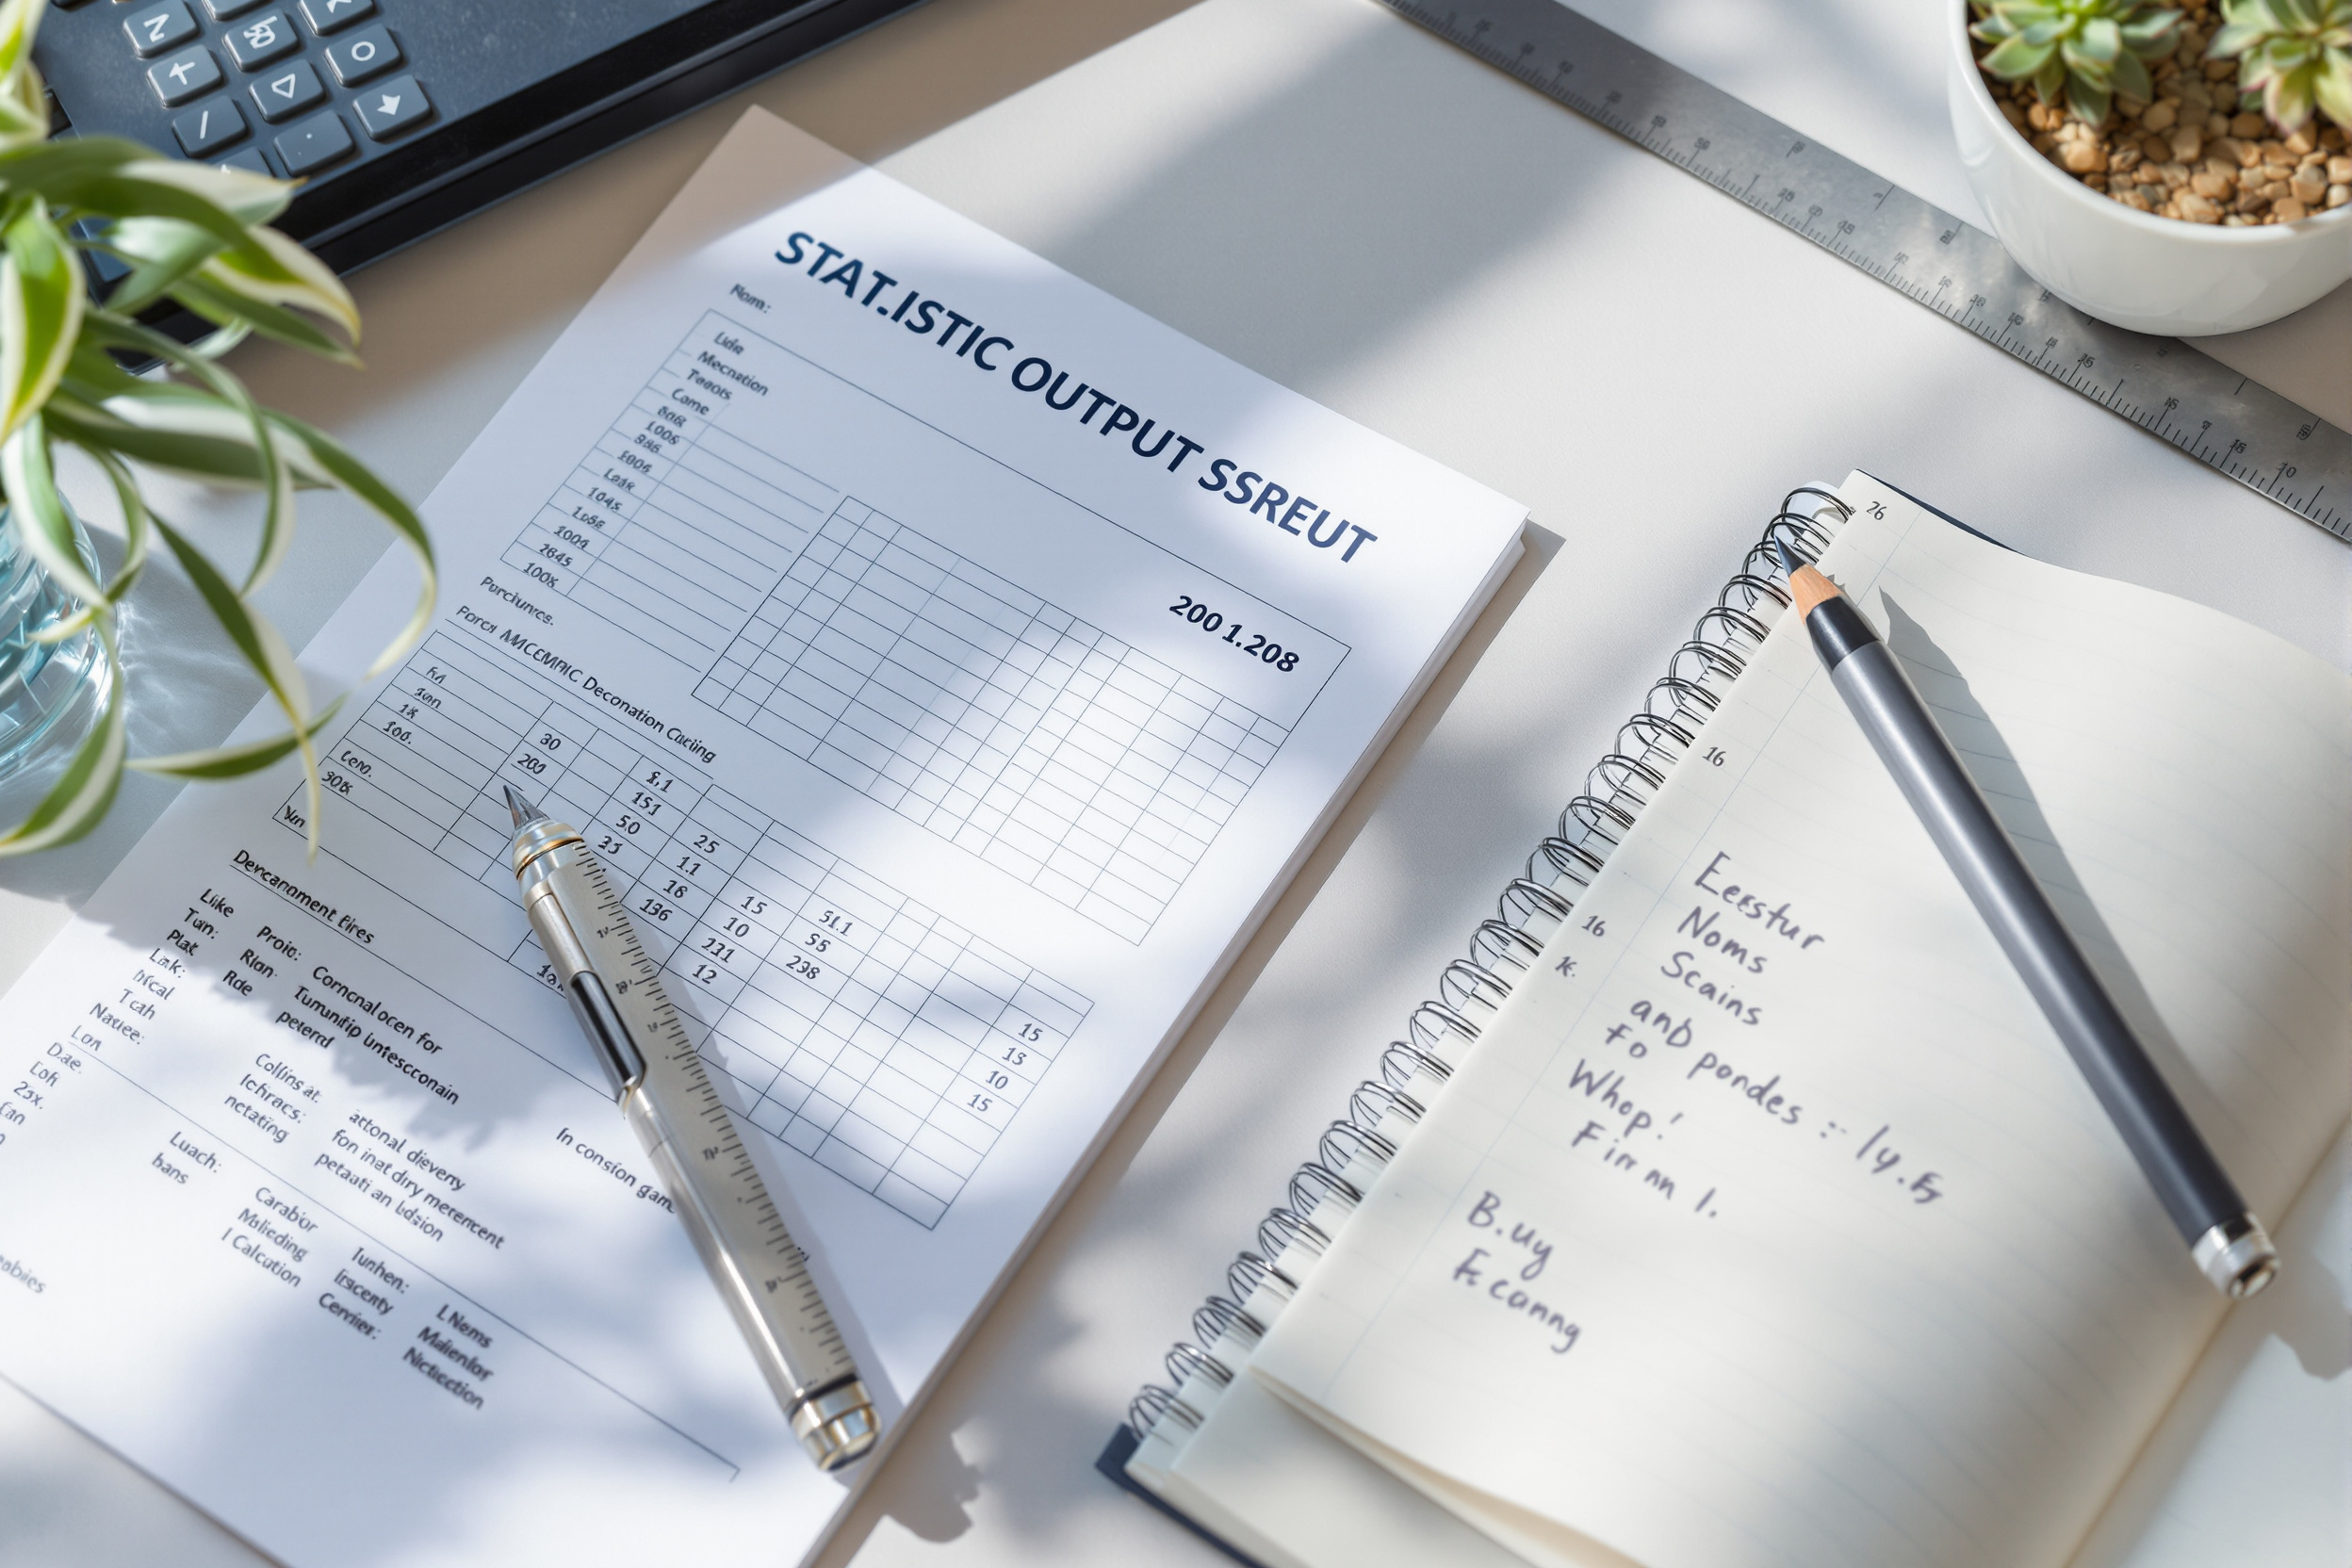
\includegraphics[width=0.85\linewidth]{images/img-cmqicyg1o000.jpg}
\caption{Świadome decyzje metodologiczne — dobór narzędzi, weryfikacja założeń i~dokumentacja procedury — stanowią o~jakości warsztatu badawczego w~pracy magisterskiej.}
\end{figure}

 Warsztat to właśnie to: świadome decyzje metodologiczne, a~nie sekwencja czynności wykonanych mechanicznie.

\begin{keyinsight}[Co recenzent sprawdza jako pierwsze]
Recenzenci prac magisterskich z~psychologii najczęściej zaczynają od hipotez i~narzędzi. Sprawdzają: czy hipotezy są operacyjne, czy skale mają polskie adaptacje o~udokumentowanych właściwościach psychometrycznych, czy analiza statystyczna jest adekwatna do poziomu pomiaru zmiennych. Te trzy elementy decydują o~tym, czy recenzja będzie zawierać pytania do wyjaśnienia na obronie, czy pochwałę warsztatu.
\end{keyinsight}

\section{Analiza wyników i~statystyka: co pokazywać, a~czego nie interpretować w~tym rozdziale}

Rozdział z~wynikami jest jedynym miejscem w~pracy magisterskiej, gdzie obowiązuje zasada absolutna: opisujesz to, co znalazłeś, nie to, co to oznacza. Interpretacja, porównanie z~literaturą, wnioski --- wszystko to należy do dyskusji.

\begin{figure}[h]
\centering

\includegraphics[width=0.85\linewidth]{images/img-cmqicymxa001.jpg}
\caption{Rozdział wyników wymaga ścisłego oddzielenia prezentacji danych od ich interpretacji, która należy wyłącznie do dyskusji.}
\end{figure}

 W~rozdziale wyników Twoim jedynym zadaniem jest rzetelna i~kompletna prezentacja tego, co pokazały analizy.

\bignumber{APA\,7}{standard raportowania wyników w~psychologii naukowej, obowiązujący na wszystkich uczelniach objętych tą książką}

Zasada ta sprawia więcej trudności, niż mogłoby się wydawać. Granica między ,,wynik'' a~,,interpretacja'' jest nieoczywista. ,,Kobiety uzyskały istotnie wyższe wyniki na skali empatii emocjonalnej ($t(198) = 3{,}12$, $p = 0{,}002$, $d = 0{,}44$)'' --- to wynik. ,,Kobiety są bardziej empatyczne, co potwierdzają wcześniejsze badania i~może wynikać z~różnic w~socjalizacji'' --- to interpretacja, która do dyskusji, nie do wyników.

\subsection{Struktura rozdziału wyników}

Rozdział wyników w~pracy magisterskiej z~psychologii organizuje się zazwyczaj w~czterech krokach.

\stepflow{Statystyki opisowe, Weryfikacja założeń, Testowanie hipotez, Analizy uzupełniające}

\textbf{Statystyki opisowe.} Zacznij od charakterystyki rozkładu zmiennych: średnie, odchylenia standardowe, minimum, maksimum, ewentualnie skośność i~kurtoza, jeśli są istotne dla dalszych analiz. Standardem APA 7 jest podawanie tych wartości do dwóch miejsc po przecinku, z~wyjątkiem wartości $p$, którą podajesz do trzech miejsc po przecinku. Statystyki opisowe umieszcza się w~tabeli, jeśli obejmują więcej niż trzy zmienne --- w~innym przypadku można je przedstawić w~tekście.

\textbf{Weryfikacja założeń.} Jeśli planujesz testy parametryczne, tutaj raportujesz wyniki testów założeń. Normalność rozkładu: wyniki testu Shapiro-Wilka dla małych prób (do 50 osób) albo Kołmogorowa-Smirnowa dla większych. Jednorodność wariancji: test Levene'a. Jeśli założenia nie są spełnione, raportujesz zastosowaną korektę lub wskazujesz, że przeszedłeś do testów nieparametrycznych, wraz z~uzasadnieniem.

\textbf{Testowanie hipotez.} Każdą hipotezę testujesz oddzielnie i~raportujesz wynik w~standardowym formacie. Standard APA 7, opisany szczegółowo przez Pogotowie Statystyczne, wymaga podania: wartości statystyki testowej, stopni swobody, wartości $p$ (dokładnej, nie ,,p < 0,05'', z~wyjątkiem wartości mniejszych niż 0,001), oraz miary wielkości efektu. Ta ostatnia jest elementem, który studentom najczęściej umyka, a~który komisja zawsze sprawdza.

\begin{table}[ht]
\centering
\caption{Miary wielkości efektu stosowane w~psychologii --- progi interpretacyjne według Cohena}
\begin{tabularx}{\textwidth}{lXXX}
\toprule
\rowcolor{tableheadbg} \textcolor{tableheadfg}{\textbf{Miara}} & \textcolor{tableheadfg}{\textbf{Mały efekt}} & \textcolor{tableheadfg}{\textbf{Średni efekt}} & \textcolor{tableheadfg}{\textbf{Duży efekt}} \\
\midrule
$d$ Cohena (różnice między grupami) & $0{,}20$ & $0{,}50$ & $0{,}80$ \\
$r$ Pearsona (korelacja) & $0{,}10$ & $0{,}30$ & $0{,}50$ \\
$\eta^2$ (ANOVA) & $0{,}01$ & $0{,}06$ & $0{,}14$ \\
$\omega^2$ (ANOVA, mniej obciążone) & $0{,}01$ & $0{,}06$ & $0{,}14$ \\
$f^2$ (regresja) & $0{,}02$ & $0{,}15$ & $0{,}35$ \\
\bottomrule
\end{tabularx}
\end{table}

Praktyczny przykład zapisu zgodnego z~APA 7 dla korelacji: ,,Zaobserwowano istotny dodatni związek między ruminacją a~intensywnością objawów depresyjnych ($r(148) = 0{,}52$, $p < 0{,}001$)''. Dla testu $t$: ,,Osoby w~grupie eksperymentalnej uzyskały istotnie niższe wyniki na skali lęku stanu po interwencji w~porównaniu z~grupą kontrolną ($t(96) = 2{,}84$, $p = 0{,}005$, $d = 0{,}57$)''. Zwróć uwagę na zapis kursywą symboli statystycznych ($r$, $t$, $p$, $M$, $SD$) --- wymóg formalny APA 7, który w~drukowanej pracy odróżnia symbol od zwykłego tekstu.

\subsection{Tabele i~wykresy}

Tabela i~wykres nie powielają informacji zawartych w~tekście --- to kolejna zasada APA 7, którą łatwo złamać, a~trudno naprawić. Jeśli wartości średnich i~odchyleń standardowych przedstawiasz w~tabeli, w~tekście piszesz ,,Statystyki opisowe dla wszystkich zmiennych zawiera Tabela~1'' i~nie powtarzasz liczb. Jeśli rysunek przedstawia interakcję między dwiema zmiennymi, w~tekście opisujesz jej charakter słownie, bez cytowania konkretnych wartości z~wykresu.

Zgodnie z~wymogami APA 7, obowiązującymi na Wydziale Psychologii UŁ i~Instytucie Psychologii UWr, tabele mają tytuł i~numer umieszczone \emph{nad} tabelą, a~rysunki --- \emph{pod} rysunkiem. Nie stosuje się linii pionowych w~tabelach. Nagłówki kolumn są wyśrodkowane, zawartość pierwszej kolumny jest wyrównana do lewej.

\begin{tipbox}[Wykresy w~SPSS i~jamovi: czego nie wklejać]
Wykresy generowane automatycznie przez SPSS i~jamovi wymagają edycji przed umieszczeniem w~pracy. Dotyczy to przede wszystkim: usunięcia domyślnego tła siatki, opisania osi w~języku polskim, zwiększenia rozmiaru czcionki do czytelnego przy wydruku A4, oraz usunięcia legendy tam, gdzie nie jest niezbędna. Wklejanie surowego wydruku z~oprogramowania statystycznego jest wymieniane w~wytycznych Instytutu Psychologii UWr jako błąd formalny, który wymaga poprawy.
\end{tipbox}

\subsection{Wyniki nieistotne statystycznie też raportuje się}

Standard APA 7 wymaga raportowania wszystkich wyników, zarówno istotnych, jak i~nieistotnych statystycznie. W~pracy magisterskiej oznacza to, że jeśli hipoteza nie znalazła potwierdzenia, raportuje się wynik testu tak samo, jak w~przypadku potwierdzenia --- ze statystyką, stopniami swobody, wartością $p$ i~miarą wielkości efektu. Przemilczenie nieistotnych wyników jest traktowane jako poważne uchybienie, szczególnie gdy recenzent zadaje na obronie pytanie: ,,A co z~hipotezą drugą?''

\begin{warningbox}[Błąd selekcji wyników]
Przedstawianie wyłącznie hipotez, które uzyskały potwierdzenie, i~pomijanie milczeniem tych, które nie uzyskały, to błąd formalny --- i~naukowy. Komisja ma dostęp do metodologii, w~której wymieniłeś wszystkie hipotezy. Jeśli wyniki omawiają tylko część z~nich, recenzent zapyta o~resztę. Przygotuj opis każdego wyniku, bez względu na jego kierunek i~istotność.
\end{warningbox}

\begin{keyinsight}[Wyniki: fakty, nie interpretacje]
Rozdział z~wynikami jest skończony, gdy opisujesz każdą hipotezę z~kompletnym zestawem statystyk: wartość testu, stopnie swobody, dokładna wartość $p$, miara wielkości efektu. Jeśli czujesz potrzebę wyjaśnienia, co wynik oznacza w~kontekście literatury --- zanotuj to zdanie i~przenieś do dyskusji. Wyniki, które mają być czytelne, muszą być suche.
\end{keyinsight}

\section{Dyskusja i~wnioski: gdzie autorzy magisterek tracą oceny}

Jeśli komisja egzaminacyjna ma jeden ulubiony zarzut wobec prac magisterskich z~psychologii, brzmi on: ,,To, co Pani/Pan opisuje jako wniosek, to spekulacja''. Dyskusja jest sekcją, w~której ta granica jest najczęściej przekraczana --- i~gdzie najłatwiej ją ochronić, jeśli rozumie się, na czym ta granica polega.

\concept{Wniosek a~spekulacja}{Wniosek to twierdzenie bezpośrednio wynikające z~zebranych danych, sformułowane z~uwzględnieniem ograniczeń badania. Spekulacja to twierdzenie wykraczające poza zgromadzone dowody, nieuzasadnione ani wynikami, ani aktualną literaturą.}

\subsection{Jak zbudować dyskusję}

Dyskusja ma odwrotną strukturę niż przegląd literatury. Tamten szedł od ogółu do szczegółu --- od szerokiego kontekstu do precyzyjnych hipotez. Dyskusja idzie od szczegółu do ogółu --- od konkretnych wyników do ich znaczenia dla teorii i~praktyki.

\stepflow{Podsumowanie wyników, Konfrontacja z~literaturą, Wyjaśnienie rozbieżności, Ograniczenia, Wnioski i~aplikacje}

\textbf{Podsumowanie wyników.} Pierwsze akapity dyskusji streszczają kluczowe wyniki --- bez liczb i~statystyk, które były już w~poprzednim rozdziale. Chodzi o~to, żeby czytelnik, który przeczytał dyskusję bez rozdziału wyników, wiedział, co badanie pokazało. Jedno do dwóch zdań na każdą hipotezę wystarczy.

\textbf{Konfrontacja z~literaturą.} To serce dyskusji. Dla każdego wyniku pokazujesz, jak wpisuje się on w~istniejący stan wiedzy: czy potwierdza wcześniejsze badania, czy jest z~nimi sprzeczny, czy rozszerza je o~nowy kontekst. Jeśli wyniki potwierdzają hipotezy i~są zgodne z~literaturą --- dobrze, ale to dopiero połowa zadania. Musisz pokazać, co nowego wnosi Twoje badanie do istniejącego obrazu, bo samo potwierdzenie jest słabym argumentem za oryginalnością.

\textbf{Wyjaśnienie rozbieżności.} To miejsce, w~którym autorzy prac magisterskich najczęściej popełniają błąd spekulacji. Wyobraź sobie, że Twoje badanie nie znalazło oczekiwanej korelacji między stylem przywiązania a~satysfakcją ze związku, choć wcześniejsze prace tę korelację dokumentowały. Możliwe wyjaśnienia są dwa: albo efekt nie istnieje w~Twojej grupie, albo Twoje badanie miało cechy, które utrudniły jego wykrycie (za mała próba, specyfika rekrutacji, inne narzędzia pomiarowe). Wskazanie tych możliwości jako hipotez wyjaśniających to dyskusja naukowa. Stwierdzenie, że ,,wyniki te mogą oznaczać, że styl przywiązania jest mniej ważny niż wcześniej sądzono'' --- bez żadnego oparcia w~danych --- to spekulacja.

\begin{examplebox}[Jak rozbieżność zamienić w~argument]
Typowa sytuacja: badanie satysfakcji zawodowej wśród psychologów pracujących w~ochronie zdrowia nie wykazało oczekiwanego związku między wsparciem społecznym a~wypaleniem zawodowym --- podczas gdy meta-analiza z~2020 roku objęła ten związek jako jeden z~najsilniejszych efektów w~obszarze. Dobra dyskusja wygląda tak: wskazujesz, że próba w~Twoim badaniu była rekrutowana wyłącznie z~placówek publicznych, gdzie struktury wsparcia formalnego są zunifikowane, co mogło ograniczyć zmienność predyktora. Podajesz, że próba liczyła 74 osoby, podczas gdy moc testowana post hoc w~G*Power wyniosła $0{,}62$ --- poniżej zalecanego $0{,}80$. Następnie wskazujesz, że przyszłe badania powinny objąć pracowników z~sektora prywatnego i~zwiększyć próbę. To jest dyskusja: dane, ograniczenia, kierunki. Nie spekulacja: dane, domysły, uogólnienia.
\end{examplebox}

\subsection{Ograniczenia badania}

Ograniczenia to element, który studenci piszą albo zbyt skromnie (jedno zdanie o~,,małej próbie''), albo zbyt szeroko (lista wszystkich możliwych problemów metodologicznych istniejących w~psychologii). Właściwa forma jest między tymi skrajnościami.

Ograniczenia powinny dotyczyć Twojego konkretnego badania, a~nie ogólnych problemów metodologii. ,,Badanie miało charakter korelacyjny, co uniemożliwia wnioskowanie przyczynowe'' --- to standardowe ograniczenie, które dotyczy połowy badań w~psychologii i~samo w~sobie niczego nie mówi o~Twojej pracy. ,,Korelacyjny charakter badania uniemożliwia rozstrzygnięcie, czy to ruminacja nasila objawy depresyjne, czy odwrotnie --- ten kierunek zależności pozostaje przedmiotem dyskusji w~literaturze i~wymagałby weryfikacji w~badaniu longitudinalnym lub eksperymentalnym'' --- to ograniczenie, które wskazuje konkretny problem interpretacyjny i~proponuje kierunek jego rozwiązania.

Ograniczenia dotyczące próby, narzędzi i~procedury powinny być powiązane z~wnioskami o~zakresie generalizacji. Jeśli badałeś studentów psychologii rekrutowanych przez ogłoszenie w~mediach społecznościowych, wniosek o~tym, jak self-selection bias mógł wpłynąć na wyniki, jest merytoryczny. Jeśli badałeś pacjentów jednej poradni w~jednym mieście, ograniczenie geograficzne i~instytucjonalne generalizacji jest uzasadnione.

\subsection{Wnioski i~aplikacje praktyczne}

Wnioski w~pracy magisterskiej z~psychologii mają dwa poziomy. Pierwszy --- teoretyczny: co wyniki mówią o~mechanizmach badanego zjawiska, jak wpisują się w~istniejące modele, które z~konkurujących wyjaśnień uzyskują wsparcie. Drugi --- praktyczny: co wyniki mogą oznaczać dla psychologów pracujących w~danym obszarze.

Ten drugi poziom jest mile widziany przez komisję, ale wymaga ostrożności. Wnioski praktyczne muszą wynikać z~wyników, nie z~osobistych przekonań autora. ,,Wyniki sugerują, że interwencje ukierunkowane na regulację emocji mogą być skuteczniejsze w~redukcji prokrastynacji akademickiej niż strategie zarządzania czasem'' --- to wniosek oparty na wynikach wskazujących na emocjonalne uwarunkowania prokrastynacji. ,,Należy zmienić programy nauczania, żeby uwzględniały regulację emocji'' --- to daleko idące zalecenie polityki edukacyjnej, niezakorzenione w~danych z~jednego badania przekrojowego na studentach.

\begin{warningbox}[Gdzie kończy się wniosek, a~zaczyna spekulacja]
Jeśli jesteś w~stanie wskazać konkretny wynik ze swojego badania, który daje podstawę dla każdego zdania w~sekcji wniosków --- jesteś bezpieczny. Jeśli zdanie w~wnioskach jest prawdziwe, ale nie wynika z~żadnego konkretnego wykresu, tabeli ani statystyki z~Twojej pracy --- to spekulacja. Test jest prosty: ,,Skąd to wiem?'' Jeśli odpowiedź to ,,z literatury'' albo ,,to logiczne'' --- zdanie należy do dyskusji, nie do wniosków, albo powinno zostać usunięte.
\end{warningbox}

\subsection{Jak nie kończyć dyskusji}

Ostatni akapit dyskusji --- i~całej pracy --- jest tym, który komisja przeczyta z~uwagą. Złe zakończenia są powtarzalne: albo to podsumowanie streszczenia, które było już we wstępie, albo ogólny komentarz o~tym, że ,,badania nad tym zjawiskiem powinny być kontynuowane''. Dobre zakończenie wskazuje jeden konkretny kierunek przyszłych badań wynikający z~ograniczeń badania, i~jedno konkretne stwierdzenie o~tym, co badanie wniosło do rozumienia zjawiska.

Instytut Psychologii UWr zaleca pisanie tekstu w~trybie oznajmującym, a~dyskusję --- podobnie jak przegląd literatury --- w~czasie teraźniejszym. Tylko opis przeprowadzonego badania i~jego wyników pisany jest w~czasie przeszłym. Ta zasada jest zaskakująco często ignorowana przez studentów, którzy piszą dyskusję w~czasie przeszłym przez analogię do wyników. Komisja to widzi.

\pullquote{Dyskusja to nie miejsce na to, co chciałeś znaleźć. To miejsce na to, co znalazłeś --- i~na uczciwe wyjaśnienie, dlaczego wynik wygląda tak, a~nie inaczej.}

\begin{keyinsight}[Granica między wnioskiem a~spekulacją]
Każde twierdzenie w~dyskusji i~wnioskach musi mieć zakotwiczenie: albo w~konkretnym wyniku z~Twojego badania, albo w~cytowanej literaturze, albo wprost opisane jako hipoteza wymagająca weryfikacji. Twierdzenia bez zakotwiczenia --- nawet intuicyjnie przekonujące --- to spekulacja. Komisja nie kwestionuje intuicji; kwestionuje twierdzenia, których nie da się obronić danymi. Rozróżnienie między tymi dwoma kategoriami jest tym, co oddziela prace oceniane na piątkę od tych, które kończą się długą listą pytań na obronie.
\end{keyinsight}

\section{Formatowanie tekstu naukowego: standardy, których nie warto negocjować}

Pisanie rozdziałów to nie tylko kwestia treści --- to również forma, w~jakiej ta treść dociera do recenzenta. Komisja egzaminacyjna ocenia pracę jako całość: argumentację i~jej opakowanie. Niespójne formatowanie nie dyskwalifikuje pracy, ale sygnalizuje brak dbałości o~szczegóły, co w~psychologii naukowej ma znaczenie: metodologia zbudowana na szczegółach musi być opisana przez kogoś, kto na szczegóły zwraca uwagę.

APA 7 --- standard obowiązujący w~psychologii akademickiej na polskich uczelniach --- określa formatowanie precyzyjniej, niż większość studentów zdaje sobie sprawę przed napisaniem pierwszego rozdziału. Czcionka może być Times New Roman 12~pt, Georgia 11~pt, Calibri 11~pt lub Arial 11~pt. Wybór należy do studenta, ale musi być jednolity w~całej pracy: ten sam krój w~tekście głównym, tabelach, opisach rycin i~bibliografii. Marginesy wynoszą 2{,}5~cm z~każdej strony. Interlinia to podwójny odstęp, bez wyjątków --- dotyczy również bibliografii i~opisów tabel.

\subsection{Poziomy śródtytułów i~ich praktyczne zastosowanie}

APA 7 definiuje pięć poziomów śródtytułów. W~pracy magisterskiej z~psychologii zazwyczaj wystarczają trzy. Poziom pierwszy to główne rozdziały: wyśrodkowany, pogrubiony, pierwsza litera tytułu wielka. Poziom drugi to podrozdziały: wyrównany do lewej, pogrubiony. Poziom trzeci: wyrównany do lewej, pogrubiony, kursywa. Każdy poziom niższy powinien pojawiać się tylko wtedy, gdy jest ich co najmniej dwa w~obrębie nadrzędnego działu --- śródtytuł bez pary wygląda strukturalnie dziwnie i~sugeruje, że podział mógł być zbędny.

Śródtytuły w~polskich pracach pisanych według APA 7 mają jedną adaptację względem wersji anglojęzycznej: wielką literą piszemy tylko pierwsze słowo tytułu (i~nazwy własne), nie wszystkie ważne słowa jak w~oryginale angielskim. Wytyczne Instytutu Psychologii UŁ explicite to zaznaczają i~traktują jako element oceny edytorskiej pracy.

\begin{tipbox}[Numeracja śródtytułów: kiedy warto, kiedy nie]
APA 7 zaleca brak numeracji śródtytułów w~artykułach naukowych. W~pracach zwartych --- w~tym w~pracy magisterskiej --- Skimina, Harasimczuk i~Cieciuch dopuszczają numerację, jeśli zwiększa czytelność i~ułatwia nawigację po tekście. Jeśli Twoja praca ma skomplikowaną strukturę z~wieloma poziomami podrozdziałów, numeracja w~stylu 1., 1.1., 1.1.1. może być pomocna. Jeśli struktura jest prosta --- numeracja nie jest potrzebna i~może sprawiać wrażenie sztucznego zagęszczenia tekstu.
\end{tipbox}

\subsection{Liczebniki i~ich zapis}

Zasada zapisu liczebników w~APA 7 jest prosta w~swojej ogólnej formie, ale ma tyle wyjątków, że warto ją przyswoić przed pisaniem rozdziału wyników. Liczebniki poniżej dziesięciu zapisuje się słownie, pozostałe cyframi. Wyjątki obejmują: bezpośrednie poprzedzanie jednostki pomiaru (zawsze cyframi: 5~cm, 3~ml), wyniki statystyczne i~procenty (zawsze cyframi: 74\% próby, współczynnik $\alpha = 0{,}87$), wiek, wyniki na skalach i~sumy punktów (zawsze cyframi). Zdania nigdy nie zaczyna się cyfrą --- jeśli jest to konieczne, liczbę zapisuje się słownie.

Zapis dziesiętny w~języku polskim używa przecinka jako separatora, nie kropki. Oznacza to, że \mbox{$p = 0{,}034$} jest poprawne, a~$p = 0.034$ --- nie. W~pracach pisanych po polsku według standardu APA 7 ten zapis jest szczegółem, który recenzenci z~doświadczeniem w~analizie danych sprawdzają odruchowo.

\section{Cytowania i~bibliografia: pułapki, których można uniknąć}

Cytowania to element pracy magisterskiej, w~którym błędy popełniane są mechanicznie --- nie ze złej woli, lecz z~braku nawyku konsekwentnego sprawdzania. Komisja egzaminacyjna rzadko weryfikuje każde cytowanie podczas obrony, ale recenzent czytający pracę przed obroną te błędy widzi i~odnotowuje.

\concept{Cytowanie w~tekście vs.\ pozycja bibliograficzna}{Każde odwołanie do cudzych idei w~tekście musi mieć odpowiadającą pozycję w~bibliografii. Każda pozycja w~bibliografii musi mieć co najmniej jedno odwołanie w~tekście. Bibliografa zawierająca pozycje, do których praca się nie odwołuje, i~tekst zawierający odwołania bez pozycji w~bibliografii --- oba są błędami formalnymi.}

\subsection{Format odwołań w~tekście}

Odwołanie do jednego autora: ,,jak wskazuje Kowalski (2018)'' albo ,,wyniki badań potwierdzają tę zależność (Kowalski, 2018)''. Dwóch autorów: za każdym razem podaje się oba nazwiska, połączone ,,i'' w~tekście ciągłym albo ,,;'' w~nawiasie. Trzech i~więcej autorów: od pierwszego odwołania stosuje się formę ,,Kowalski i~in.'' --- to zmiana wprowadzona w~APA 7 względem poprzedniej edycji, która wymagała pełnego zestawu nazwisk przy pierwszym cytowaniu. Studenci, którzy korzystają z~poradników opartych na APA 6, popełniają tutaj błąd.

Cytowanie bezpośrednie --- dosłowne przytoczenie fragmentu tekstu --- wymaga podania strony. Fragment do 40 słów umieszcza się w~cudzysłowie w~tekście ciągłym. Powyżej 40 słów: wyodrębniony akapit z~powiększonym lewym marginesem. Instytut Psychologii UWr wskazuje, że w~całej pracy bezpośrednie cytaty nie powinny przekraczać 5 procent objętości. W~pracach empirycznych z~psychologii ten limit jest zazwyczaj osiągany jedynie przez autorów, którzy cytują narzędzia pomiarowe lub instrukcje dosłownie --- co ma uzasadnienie. Cytowanie cudzych argumentów teoretycznych słowo w~słowo zamiast parafrazowania to błąd jakościowy, nie tylko formalny.

\begin{warningbox}[Cytowanie za pośrednictwem bez dostępu do oryginału]
Jeśli artykuł A~przywołuje wyniki badania B, a~Ty nie dotarłeś do B bezpośrednio, nie cytuj B tak, jakbyś go przeczytał. Prawidłowy zapis: ,,jak wykazali Smith i~Jones (2010, za: Kowalski, 2018)''. W~bibliografii umieszczasz tylko Kowalskiego (2018), nie Smitha i~Jonesa. Cytowanie pracy, której nie czytałeś, jako czytanej jest błędem akademickim --- nie tylko formalnym. Jeśli wyniki badania B są kluczowe dla Twojego argumentu, znajdź oryginał.
\end{warningbox}

\subsection{Format bibliografii}

Bibliografię w~stylu APA 7 organizuje się alfabetycznie według nazwiska pierwszego autora, bez podziału na typy źródeł. Interlinia jest podwójna --- tak samo jak w~tekście głównym. Wcięcie stosuje się odwrócone: pierwszy wiersz każdej pozycji bez wcięcia, kolejne wiersze z~wcięciem jednego tabulatora. Tytuły artykułów w~czasopismach pisane są zwykłą czcionką bez cudzysłowu; nazwy czasopism --- kursywą, z~numerem tomu (również kursywą) i~numerem zeszytu w~nawiasie (bez kursywy).

Przykładowy zapis artykułu w~czasopiśmie: Kowalska, A., i~Nowak, B. (2021). Regulacja emocji a~prokrastynacja akademicka: mediacyjna rola unikania doświadczeniowego. \textit{Psychologia Społeczna, 16}(3), 245--261.

Przykładowy zapis książki: Wrześniewski, K. (2009). \textit{Psychologiczne uwarunkowania powstawania i~przebiegu choroby niedokrwiennej serca}. Wydawnictwo Naukowe UAM.

Przykładowy zapis rozdziału w~pracy zbiorowej: Oleś, P. (2011). Tożsamość a~narracja. W: B. de Barbaro, C. Skowrońska-Jóźwiak i~B. Józefik (red.), \textit{Koncepcja narracyjna siebie} (s.~23--45). Wydawnictwo Uniwersytetu Jagiellońskiego.

\begin{tipbox}[Menedżery bibliografii w~pracy magisterskiej z~psychologii]
Zotero i~Mendeley automatycznie formatują cytowania i~bibliografię w~stylu APA 7, ale wyniki ich pracy wymagają weryfikacji. Szczególnie w~pracach polskojęzycznych systemy te generują błędy: wstawiają ,,\&'' zamiast ,,i'' w~odwołaniach w~tekście, używają angielskich skrótów (,,et al.'' zamiast ,,i~in.''), a~czasami niepoprawnie formatują artykuły z~polskich czasopism. Menedżer bibliografii to narzędzie wspomagające, nie zastępujące weryfikację. Przed złożeniem pracy sprawdź każdą pozycję w~bibliografii ręcznie.
\end{tipbox}

\section{Spójność pracy jako całości: czego nie widać w~poszczególnych rozdziałach}

Praca magisterska z~psychologii jest dokumentem, który komisja czyta nie tylko sekcja po sekcji, ale też jako całość. Spójność wewnętrzna --- między pytaniami badawczymi a~hipotezami, między hipotezami a~narzędziami pomiaru, między narzędziami a~analizami, między analizami a~wnioskami --- jest tym, co odróżnia prace dobrze skonstruowane od tych, które sprawiają wrażenie sklejonych z~osobno napisanych fragmentów.

Konkretny przykład: jeśli w~pytaniu badawczym pytasz o~moderacyjną rolę płci w~związku między regulacją emocji a~prokrastynacją, a~w~rozdziale wyników tej moderacji nie testujesz --- komisja zapyta, dlaczego. Jeśli hipoteza mówi o~mediacji, a~analiza statystyczna obejmuje wyłącznie korelacje --- recenzent napisze, że metodologia jest nieadekwatna do pytania. Te niespójności trudno dostrzec, kiedy pisze się rozdziały w~różnym czasie i~różnej kolejności. Dlatego ostateczna wersja pracy wymaga przeczytania jej od początku do końca jako jednego dokumentu, z~jednym pytaniem: czy każdy element wynika logicznie z~poprzedniego?

\stepflow{Pytanie badawcze, Hipotezy, Narzędzia, Analiza statystyczna, Wyniki, Wnioski}

Każde ogniwo tego łańcucha musi być spójne z~poprzednim i~następnym. Hipotezy nie mogą testować czegoś, o~czym pytanie badawcze nie mówiło. Narzędzia muszą mierzyć zmienne wskazane w~hipotezach. Analiza musi odpowiadać poziomowi pomiaru zmiennych i~charakterowi hipotezy (kierunkowa czy bezkierunkowa, związek czy różnica, mediacja czy moderacja). Wyniki muszą dotyczyć każdej hipotezy. Wnioski muszą być zakorzenione w~wynikach.

\begin{examplebox}[Niespójność, która kosztuje ocenę]
Wyobraź sobie pracę, w~której pytanie badawcze dotyczy związku między jakością snu a~funkcjonowaniem poznawczym u~osób z~przewlekłym bólem. Hipotezy precyzują: słabsza jakość snu będzie przewidywała gorsze wyniki na testach uwagi i~pamięci roboczej. W~rozdziale narzędzi autor opisuje kwestionariusz jakości snu (PSQI) i~dwa testy neuropsychologiczne. Jak dotąd wszystko spójne. Problem pojawia się w~analizach: autor przeprowadził wyłącznie korelacje, a~hipotezy sugerują predykcję --- czyli potrzebna była regresja liniowa. Na obronie komisja zapyta, dlaczego zastosowano korelację, skoro hipotezy mówią o~przewidywaniu. Odpowiedź ,,bo korelacja też pokazuje związek'' jest merytorycznie słaba: korelacja i~regresja to różne pytania o~te same dane. Ta niespójność nie pochodzi z~braku wiedzy --- pochodzi z~braku finalnej weryfikacji całości.
\end{examplebox}

Pisanie pracy magisterskiej z~psychologii jest procesem nieliniowym: hipotezy są formułowane razem z~promotorem, narzędzia dobierane przed zebraniem danych, analiza zaplanowana z~wyprzedzeniem --- ale konkretne słowa na stronie często powstają w~różnych momentach, z~różnymi decyzjami w~tle. Finalna lektura całości, z~ołówkiem i~pytaniem o~spójność każdego elementu, to nie formalność. To ostatnia okazja, żeby praca zaprezentowała się jako spójna całość, a~nie jako suma sprawnie napisanych fragmentów.

\begin{keyinsight}[Praca jako jeden argument]
Komisja egzaminacyjna czyta pracę magisterską z~jednym nadrzędnym pytaniem: czy autor rozumie, co zrobił i~dlaczego każda podjęta decyzja --- od wyboru tematu przez dobór narzędzi po sformułowanie wniosków --- była uzasadniona. Każdy rozdział, który napisałeś, jest odpowiedzią na część tego pytania. Spójność między rozdziałami jest odpowiedzią na całość. Prace, które przechodzą obronę bez trudnych pytań, to prace, w~których każde ogniwo łańcucha badawczego trzyma się następnego.
\end{keyinsight}
\clearpage

\chapter{Obrona i~finisz: formatowanie, seminarium i~egzamin}

\lettrine{O}{statnie} tygodnie przed obroną mają osobną psychologię. Po dwóch latach pracy nagle okazuje się, że praca jest napisana, a~i~tak nie wiadomo, co z~nią zrobić: jak ją sformatować, kiedy wysłać promotorowi, co powiedzieć komisji, gdy zapyta o~ograniczenia metodologiczne. Ten rozdział jest przewodnikiem przez ten właśnie etap --- konkretnym, sekwencyjnym i~pozbawionym ogólników.

\section{Wymogi formalne i~edytorskie: co różni uczelnie, a~co jest standardem}

Większość studentów psychologii zakłada, że formatowanie to drobnostka do ogarnięcia w~ostatni weekend. To błąd, który potrafi opóźnić złożenie pracy o~kilka tygodni. Promotorzy zwracają prace z~powodów tak prozaicznych, jak nieprawidłowe wcięcia akapitów, brak numeru ORCID na stronie tytułowej albo niespójne formatowanie odsyłaczy bibliograficznych.

\concept{Standard APA 7}{Siódme wydanie \emph{Publication Manual of the American Psychological Association} (2020) to obowiązujący format dla prac psychologicznych w~Polsce. Skimina, Harasimczuk i~Cieciuch (2022) opracowali jego polską adaptację, obejmującą specyficzne zasady zapisu dla tekstów w~języku polskim --- m.in. regułę stosowania spójnika ,,i'' zamiast ,,\&'' w~odsyłaczach oraz pisownię śródtytułów małą literą.}

Standardy APA 7 obowiązują na zdecydowanej większości wydziałów psychologii w~Polsce, jednak uczelnie nakładają na nie własną warstwę wymagań. Rozbieżności dotyczą kilku obszarów: kroju i~rozmiaru czcionki (Times New Roman 12 pt lub Calibri 11 pt --- to zależy od regulaminu), szerokości marginesów (najczęściej 2,5 cm lub 3 cm od lewej), numeracji stron (niektóre uczelnie wymagają jej od strony tytułowej, inne dopiero od wstępu) oraz objętości pracy (zakres 80--120 stron jest powszechny, ale Vizja czy SWPS potrafią określić minimalną liczbę znaków ze spacjami). Zanim zaczniesz formatować, pobierz aktualny regulamin dyplomowania ze strony swojego dziekanatu --- wersja sprzed dwóch lat może już nie obowiązywać.

Niezależnie od uczelni, pięć elementów pozostaje stałych w~pracach z~psychologii.

\textbf{Śródtytuły według APA 7.} W~polskojęzycznym tekście śródtytuł 1.\ stopnia jest wyśrodkowany i~pogrubiony, a~pierwsze słowo zaczyna się wielką literą. Śródtytuł 2.\ stopnia --- wyrównany do lewej i~pogrubiony. Śródtytuł 3.\ stopnia --- wyrównany do lewej, pogrubiony i~kursywą. Śródtytuły 4.\ i~5.\ stopnia zaczynają się od wcięcia i~kończą kropką, po której tekst biegnie dalej w~tym samym wierszu. Nie numeruje się śródtytułów cyframi ani literami, a~między śródtytułem a~poprzedzającym go akapitem nie wstawia się pustego wiersza.

\textbf{Odsyłacze bibliograficzne.} Przy jednym lub dwóch autorach każdorazowo podajemy oba nazwiska. Przy trzech i~więcej --- od pierwszego cytowania stosujemy formę ,,Nowak i~in. (2021)''. Kilka prac w~jednym nawiasie porządkuje się alfabetycznie i~oddziela średnikiem: (Kowalski i~Wiśniewski, 1998; Nowak, 2021). Rok publikacji w~nawiasie pomijamy w~kolejnych odwołaniach do tej samej pracy w~obrębie jednego akapitu, o~ile kontekst jest jednoznaczny.

\textbf{Wcięcia akapitów.} Każdy akapit, łącznie z~pierwszym po śródtytule, zaczyna się wcięciem na jeden tabulator (domyślnie 1,27 cm). Wyjątki: streszczenie, cytaty powyżej 40 słów oraz pozycje w~bibliografii --- tam wcięciem objęty jest drugi i~każdy kolejny wiersz, nie pierwszy.

\textbf{Cytaty powyżej 40 słów.} Wyodrębnia się je jako osobny blok z~wcięciem 1,27 cm z~lewej strony, bez cudzysłowów, w~tym samym rozmiarze czcionki. Odsyłacz bibliograficzny z~numerem strony umieszcza się po kropce kończącej cytat.

\textbf{Tabele i~rysunki.} Tytuł tabeli umieszcza się nad nią (pogrubiony, wyrównany do lewej), tytuł rysunku --- pod nim. Każda tabela i~rysunek muszą być omówione w~tekście przed ich pojawieniem się.

\begin{warningbox}[Strona tytułowa to nie formalność]
Regulaminy precyzują kolejność elementów na stronie tytułowej: nazwa uczelni, wydział, imię i~nazwisko autora, tytuł pracy (po polsku i~angielsku), informacja o~promotorze, miejscowość i~rok. Brak angielskiego tytułu lub błędnie podana specjalność skutkuje odesłaniem pracy do poprawki --- niezależnie od jej merytorycznej jakości.
\end{warningbox}

\stepflow{Pobierz regulamin, Ustaw marginesy i~czcionkę, Sformatuj śródtytuły, Sprawdź bibliografię, Wygeneruj spis treści, Złóż w~dziekanacie}

Poniższa tabela pokazuje, gdzie uczelnie najczęściej się różnią --- i~gdzie panuje jednolity standard.

\begin{table}[ht]
\centering
\caption{Elementy formatowania: standard APA 7 a~typowe wymagania uczelniane}
\begin{tabularx}{\textwidth}{lXl}
\toprule
\rowcolor{tableheadbg} \textcolor{tableheadfg}{\textbf{Element}} & \textcolor{tableheadfg}{\textbf{Standard APA~7 / polskie wytyczne}} & \textcolor{tableheadfg}{\textbf{Zmienność uczelniana}} \\
\midrule
Czcionka & Times New Roman 12 pt lub Calibri 11 pt & Wysoka --- zależy od regulaminu \\
Interlinia & 2,0 (podwójna) & Średnia --- SWPS dopuszcza 1,5 \\
Marginesy & 2,54 cm z~każdej strony & Średnia --- część uczelni wymaga 3 cm z~lewej \\
Odsyłacze & Nazwisko, rok w~nawiasie & Niska --- APA obowiązuje wszędzie \\
Śródtytuły & Pięć stopni hierarchii & Niska --- format ustalony przez APA \\
Strona tytułowa & Brak szablonu w~APA & Wysoka --- każda uczelnia ma własny wzór \\
Objętość pracy & Brak sztywnego limitu & Wysoka --- od 60 do 120 stron \\
\bottomrule
\end{tabularx}
\end{table}

\begin{keyinsight}[Gdzie szukać aktualnych wymogów]
Regulamin dyplomowania pobierz bezpośrednio z~witryny dziekanatu --- nie polegaj na wersji przekazanej przez starszych kolegów. Polską adaptację APA~7 opracowaną przez Skiminę, Harasimczuka i~Ciecucha (2022) znajdziesz bezpłatnie pod adresem apa7.liberilibri.pl --- to 60 stron precyzyjnych reguł zapisu, które rozstrzygają każdą wątpliwość edytorską.
\end{keyinsight}

\section{Praca z~promotorem: jak zarządzać seminarium przez dwa lata}

Promotorzy nie są jednorodni. Jedni oczekują rozdziałów co miesiąc, inni wolą rzadsze, ale dopracowane wersje. Jedni odpowiadają na maile w~ciągu doby, inni --- po dwóch tygodniach. Niezależnie od stylu pracy konkretnej osoby, to student odpowiada za rytm współpracy, nie promotor. Jeśli piszesz pracę na wydziale psychologii i~seminarium magisterskie trwa dwa lata (cztery semestry) --- albo trzy semestry, jak w~programie Wizja --- masz precyzyjnie wyznaczone okna czasowe na każdy etap.

\pullquote{Promotor nie pisze za ciebie. Wskazuje kierunek --- resztę drogi przechodzisz sam.}

\textbf{Trzy semestry w~modelu Vizja.} Program seminarium magisterskiego na Vizja obejmuje trzy semestry (seminarium I, II i~III), przy czym ostatni semester jest najcięższy --- 20 punktów ECTS, 60 godzin spotkań. To nie jest przypadkowe. Ostatni semestr jest zaprojektowany jako intensywny sprint: zbierasz dane, analizujesz wyniki i~składasz gotową pracę. Jeśli nie masz do tego momentu skończonych rozdziałów teoretycznych i~zatwierdzonej metodologii, sprint zamienia się w~chaos.

W~pierwszym semestrze seminarium (zwykle drugi semestr pierwszego roku studiów) powinieneś zrealizować trzy rzeczy: wybrać i~zatwierdzić temat, napisać wstępny przegląd literatury (15--20 stron) oraz przedyskutować projekt metodologiczny z~promotorem. To jest etap, na którym promotor ma największy wpływ na kształt pracy --- i~tu warto zadawać pytania, a~nie czekać na instrukcje.

W~drugim semestrze seminarium skupiasz się na rozdziale metodologicznym i~zbieraniu danych. Do końca tego semestru powinieneś mieć: zatwierdzony schemat badań, skompletowane narzędzia pomiarowe (wraz ze zgodami na ich użycie, jeśli są wymagane), zatwierdzone zgody etyczne oraz przynajmniej wstępne dane. Promotor powinien zobaczyć rozdział metodologiczny w~wersji ,,roboczej'' --- nie czekaj z~tym do ostatniego spotkania.

Trzeci semestr to analiza, wyniki, dyskusja i~złożenie pracy. Tutaj liczy się przede wszystkim terminowość: większość uczelni wymaga złożenia pracy w~dziekanacie na 4--6 tygodni przed wyznaczonym terminem obrony. Spóźnienie o~tydzień potrafi przesunąć obronę o~cały cykl --- czyli o~pół roku.

\begin{tipbox}[Zasada 48 godzin i~krótki brief]
Wysyłając promotorowi nowy fragment pracy, zawsze dołącz krótki brief (3--5 zdań): co zmieniłeś od ostatniej wersji, o~co konkretnie prosisz (komentarz merytoryczny, ocena struktury, sprawdzenie spójności z~poprzednim rozdziałem). To skraca czas odpowiedzi i~sprawia, że uwagi są trafniejsze. Nie wysyłaj pliku bez kontekstu --- promotor prowadzi często kilkanaście seminariów równocześnie.
\end{tipbox}

Uwagi promotora bywają niekomfortowe. Zdarzają się komentarze w~stylu ,,cały ten fragment trzeba przepisać'' po trzech miesiącach pracy. Zanim zareagujesz emocjonalnie, zadaj jedno pytanie: ,,Co konkretnie jest problematyczne --- struktura, dobór źródeł, czy styl argumentacji?'' Precyzja pytania wymusza precyzję odpowiedzi i~często okazuje się, że problem dotyczy jednego akapitu, nie całego rozdziału.

Negocjowanie zakresu pracy to temat, o~którym mało kto mówi otwarcie. Jeśli w~trakcie zbierania danych okazuje się, że pierwotne założenie było zbyt ambitne (np. zaplanowano badanie na dwóch grupach klinicznych, a~rekrutacja jednej okazuje się niemożliwa), należy poinformować promotora jak najwcześniej --- nie dwa tygodnie przed oddaniem pracy, lecz w~momencie, gdy problem staje się wyraźny. Promotorzy rozumieją ograniczenia terenowe; nie rozumieją ukrywania ich do ostatniej chwili.

\begin{examplebox}[Typowy przebieg dwuletniego seminarium]
Wyobraź sobie studentkę psychologii klinicznej, która wybrała temat ,,Regulacja emocji a~nasilenie objawów depresyjnych u~młodych dorosłych''. W~pierwszym semestrze seminarium uzgodniła z~promotorem schemat korelacyjny, przygotowała przegląd literatury i~wstępnie dobrała narzędzia: skalę DERS i~BDI-II. W~drugim semestrze zebrała dane od 94 uczestników (rekrutacja trwała sześć tygodni, nie dwa --- co uwzględniła w~harmonogramie), przeprowadziła analizy w~JASP i~napisała rozdział metodologiczny. W~trzecim semestrze skupiła się na rozdziale wyników i~dyskusji, wysyłając promotorowi kolejne wersje co dwa tygodnie. Pracę złożyła pięć tygodni przed obroną. Taki rytm wymaga planowania, nie talentu.
\end{examplebox}

\begin{keyinsight}[Rytm, nie intensywność]
Najczęstszy błąd to pisanie pracy ,,zrywami'' --- przez miesiąc intensywnie, przez trzy miesiące nic. Promotorzy rozpoznają ten wzorzec natychmiast: tekst pisany w~jednym tygodniu przed terminem ma inny styl niż tekst pisany systematycznie. Ustal z~promotorem harmonogram spotkań na początku każdego semestru i~trzymaj się go, nawet jeśli nie masz gotowych materiałów do omówienia --- samo spotkanie pozwala zachować ciągłość.
\end{keyinsight}

\section{Antyplagiat i~oryginalność: granica między cytowaniem a~przepisywaniem}

Od lutego 2024 roku Jednolity System Antyplagiatowy (JSA) obsługiwany przez Ośrodek Przetwarzania Informacji wykrywa nie tylko klasyczne plagiaty, ale też fragmenty napisane przez narzędzia sztucznej inteligencji --- w~tym ChatGPT. System obejmuje wszystkie prace dyplomowe w~Polsce i~od 2019 roku przebadał ponad 1,5 miliona prac; ponad 320 tysięcy z~nich zostało ocenionych jako potencjalne plagiaty i~nie zostało zaakceptowanych przez promotorów.

\bignumber{320\,000}{prac ocenionych jako potencjalne plagiaty w~JSA od 2019 roku --- żadna nie trafiła na obronę}

Detekcja treści wygenerowanych przez AI opiera się na mierze zwanej \emph{perplexity}: im tekst bardziej przewidywalny i~szablonowy, tym niższa wartość perplexity, tym wyższe prawdopodobieństwo wygenerowania przez model językowy. JSA nie daje stuprocentowej pewności --- ostateczna decyzja zawsze należy do promotora. Jednak wynik ,,wysokie prawdopodobieństwo AI'' wymusza rozmowę, której żaden student nie chce odbywać dwa tygodnie przed obroną.

Poprawne cytowanie w~APA 7 nie jest trudne, jeśli znasz kilka reguł. Przede wszystkim: odwołanie do cudzej pracy bez dosłownego przytaczania (parafrazowanie) wymaga odsyłacza z~nazwiskiem i~rokiem, ale bez cudzysłowu i~bez numeru strony. Dosłowny cytat wymaga odsyłacza z~numerem strony. Cytat powyżej 40 słów wyodrębnia się jako blok. W~żadnym z~tych przypadków nie kopiujesz tekstu bez zaznaczenia tego w~pracy.

Szczególnym problemem w~pracach z~psychologii są \textbf{narzędzia psychometryczne}. Skale takie jak BDI-II (Beck Depression Inventory) czy STAI (State -- Trait Anxiety Inventory) są chronione prawem autorskim. Możesz je opisać, zacytować ich nazwę, podać źródło i~powołać się na badania walidacyjne --- ale nie możesz reprodukować pozycji testowych w~tekście pracy bez pisemnej zgody wydawcy (np. Pearson Assessments). W~przypisie dolnym zamieszcza się informację o~prawach autorskich zgodnie z~formatem APA: ,,Źródło: \emph{Tytuł skali}, A. Autor, rok, Wydawnictwo. Copyright rok Nazwa Właściciela Copyright. Przedrukowane za zgodą\ldots''. Jeśli korzystasz z~narzędzi na licencji Creative Commons, wystarczy odsyłacz bibliograficzny bez ubiegania się o~zgodę.

\begin{warningbox}[Parafraza nie jest bezpieczna sama w~sobie]
Zmiana kilku słów w~zdaniu to nie parafraza --- to maskowanie cytatu. Promotorzy i~recenzenci rozpoznają ten zabieg, a~JSA wykrywa podobieństwo strukturalne, nie tylko leksykalne. Prawdziwa parafraza to przetworzenie idei z~innego źródła własnymi słowami i~własną strukturą zdania --- z~odsyłaczem do oryginału.
\end{warningbox}

\begin{keyinsight}[JSA sprawdza podobieństwo, nie intencje]
Wysoki wskaźnik podobieństwa w~raporcie JSA nie musi oznaczać plagiatu --- może wynikać ze standardowych sformułowań metodologicznych lub definicji pojęć. Promotor interpretuje raport w~kontekście całej pracy. Twoim zadaniem jest upewnić się, że każde zapożyczenie --- dosłowne czy parafrazowane --- ma odsyłacz bibliograficzny i~że żaden fragment pracy nie został wygenerowany narzędziem AI bez Twojej wiedzy i~weryfikacji.
\end{keyinsight}

\section{Egzamin magisterski: pytania komisji i~jak się na nie przygotować}

Komisja egzaminacyjna w~psychologii zadaje pytania inaczej niż na obronie w~naukach ścisłych. Rzadko chodzi o~sprawdzenie wiedzy encyklopedycznej. Najczęściej chodzi o~sprawdzenie, czy rozumiesz, co zrobiłeś i~dlaczego --- i~czy potrafisz to powiedzieć bez ściągawki.

Typowe pytania można podzielić na cztery kategorie. Pierwsza to \textbf{uzasadnienie wyboru metodologii}: ,,Dlaczego zastosowała Pani schemat korelacyjny, a~nie eksperymentalny?'', ,,Dlaczego zdecydował się Pan na próbkę wygodną zamiast losowej?'' Komisja nie oczekuje, że powiesz ,,bo tak jest łatwiej''

\begin{figure}[h]
\centering

\includegraphics[width=0.85\linewidth]{images/img-cmqicyxvq001.jpg}
\caption{Egzamin magisterski przed komisją to moment, w~którym student musi wykazać się głębokim rozumieniem własnych wyborów metodologicznych.}
\end{figure}

 --- oczekuje, że wskażesz ograniczenia każdego podejścia i~wyjaśnisz, dlaczego wybrane rozwiązanie było adekwatne do pytania badawczego. Przykładowa odpowiedź na pytanie o~próbkę wygodną: ,,Próbka wygodna ogranicza możliwość uogólniania wyników na populację, co odnotowałem w~sekcji ograniczeń. Wybrałem ją ze względów praktycznych rekrutacyjnych, a~jej jednorodność demograficzna stanowi zarazem kontrolę dla zmiennych zakłócających takich jak wiek i~poziom wykształcenia.''

Druga kategoria to \textbf{ograniczenia badania}. Komisja pyta o~nie nie po to, żeby zdyskredytować pracę, lecz żeby sprawdzić, czy student ma dojrzałą refleksję naukową. Prace, w~których sekcja ograniczeń nie istnieje albo liczy dwa zdania, są odbierane jako niedojrzałe metodologicznie. Przygotuj trzy do czterech ograniczeń swojego badania i~do każdego przyporządkuj implikację: co to ograniczenie oznacza dla interpretacji wyników i~w~jaki sposób mogłoby je zniwelować przyszłe badanie.

Trzecia kategoria to \textbf{implikacje kliniczne lub aplikacyjne}. ,,Co z~tego wynika dla praktyki psychologicznej?'' --- to pytanie pada na niemal każdej obronie w~psychologii klinicznej lub zdrowia. Odpowiedź powinna być konkretna i~osadzona w~danych: ,,Wyniki sugerują, że interwencje ukierunkowane na regulację emocji mogą być skuteczniejszym punktem wejścia do terapii depresji u~młodych dorosłych niż interwencje nastawione wyłącznie na redukcję objawów. Mój wynik korelacji $r = 0{,}58$ między trudnościami w~regulacji emocji a~nasileniem depresji jest zbliżony do wartości raportowanych przez Gruber i~współpracowników (2014), co wzmacnia spójność tego wniosku.''

Czwarta kategoria to pytania \textbf{z teorii i~literatury}: ,,Jak Pana wyniki odnoszą się do teorii regulacji emocji Grossa?'', ,,Czy zna Pani alternatywne modele wyjaśniające ten mechanizm?'' Tutaj komisja sprawdza, czy praca jest zakorzeniona w~literaturze --- a~nie czy student nauczył się jej na pamięć dwa dni przed obroną.

\begin{tipbox}[Technika ,,trzy zdania i~pytanie zwrotne'']
Gdy nie wiesz, jak odpowiedzieć na pytanie komisji, zastosuj trójkrok: (1) powiedz, co wiesz na pewno (jedno zdanie), (2) zaznacz granicę swojej wiedzy (,,W mojej pracy nie analizowałem tego aspektu, ponieważ\ldots''), (3) zaproponuj, skąd odpowiedź mogłaby wynikać (,,Sądzę, że kluczowe byłoby tu odwołanie do badań nad\ldots''). Komisja docenia samowiedzę bardziej niż improwizowane odpowiedzi.
\end{tipbox}

Co obniża ocenę obrony? Pięć rzeczy. Po pierwsze, nieznajomość własnej metodologii --- student, który nie potrafi wyjaśnić, dlaczego wybrał konkretny test statystyczny, sygnalizuje, że analizy robił ktoś inny. Po drugie, brak sekcji ograniczeń lub zdawkowe jej traktowanie. Po trzecie, niespójność między pytaniem badawczym, hipotezami a~wnioskami --- komisja często pyta wprost: ,,Jak Pana hipoteza H2 ma się do wyniku, który opisuje Pani na stronie 67?'' Po czwarte, nieumiejętność odróżnienia wyników od dyskusji --- zdarzają się studenci, którzy na pytanie o~wyniki cytują wnioski, a~na pytanie o~dyskusję --- liczby. Po piąte, defensywność: komisja zadaje trudne pytania z~życzliwości, nie złośliwości. Student, który reaguje na każde pytanie spięciem lub monosylabami, sam utrudnia sobie obronę.

\begin{examplebox}[Jak wygląda dobra obrona w~psychologii klinicznej]
Wyobraź sobie studenta, który zbadał związek między stylem przywiązania a~wypaleniem zawodowym u~pielęgniarek. Komisja pyta: ,,Dlaczego nie przeprowadził Pan analizy mediacji?'' Odpowiedź dobra: ,,Analiza mediacji wymagałaby co najmniej 200 uczestników, żeby zachować moc statystyczną na poziomie 0,80 przy efekcie małej wielkości. Moja próba liczyła 112 osób, co wystarczyło do testowania korelacji, ale nie do modelu mediacyjnego. Wskazałem to jako kierunek przyszłych badań.'' Komisja kiwa głowami --- student wie, co robi i~dlaczego tego nie zrobił. Obrona kończy się oceną bardzo dobrą.
\end{examplebox}

\stepflow{Przeczytaj pracę od nowa, Wypisz ograniczenia, Przygotuj uzasadnienie metodologii, Przećwicz odpowiedzi, Sprawdź spójność hipotez z~wnioskami, Obrona}

\begin{keyinsight}[Komisja szuka refleksji, nie perfekcji]
Żadna praca magisterska nie jest doskonała --- komisja o~tym wie. Szuka studenta, który rozumie, co zrobił, dlaczego tak zrobił i~co zrobiłby inaczej. Trzy precyzyjne ograniczenia badania z~uzasadnieniem robią lepsze wrażenie niż praca bez żadnych ograniczeń albo z~ograniczeniami skopiowanymi z~artykułów.
\end{keyinsight}

\section{Zamiast zakończenia: osiem tygodni, które mają znaczenie}

Cztery rozdziały tej książki przeprowadziły cię przez cały cykl pracy magisterskiej z~psychologii: od wyboru tematu, przez konstruowanie metodologii i~pisanie kolejnych rozdziałów, aż do formatowania i~egzaminu. Pora zamknąć ten cykl konkretnym planem.

Osiem tygodni przed obroną to optimum, w~którym wszystko jest jeszcze możliwe do naprawienia. Tydzień 1--2: finalizacja tekstu i~wysłanie do promotora z~prośbą o~ostatnie uwagi. Tydzień 3: naniesienie poprawek i~formatowanie zgodne z~regulaminem. Tydzień 4: złożenie pracy w~systemie antyplagiatowym --- zrób to sam, nie czekaj na dziekanat. Tydzień 5: złożenie w~dziekanacie, uzyskanie recenzji. Tydzień 6--7: lektura recenzji, przygotowanie odpowiedzi na potencjalne pytania komisji. Tydzień 8: próbna obrona z~promotorem lub znajomymi, ostateczne przejrzenie pracy.

Wróć do rozdziału pierwszego tej książki, gdy będziesz pisać wstęp końcowy pracy --- bo dobry wstęp powstaje na końcu, gdy już wiesz, co udowodniłeś. Wróć do rozdziału drugiego, gdy komisja zapyta o~metodologię --- tam znajdziesz argumenty, które pomogły ci ją wybrać. Wróć do rozdziału trzeciego, gdy recenzent podniesie zarzuty do dyskusji --- tam opisałem, jak dyskusja psychologiczna powinna odnosić się do literatury, nie tylko do własnych wyników.

\pullquote{Praca magisterska z~psychologii to nie dowód twojej wiedzy. To dowód, że potrafisz postawić pytanie, zebrać dane i~wyciągnąć z~nich wnioski --- z~metodologiczną uczciwością.}

Największy błąd, jaki można popełnić na tym etapie, to czekanie na idealny moment do działania. Idealne warunki do pisania nie istnieją. Istnieją tygodnie, w~których piszesz po dwie strony dziennie, i~tygodnie, w~których nie piszesz nic --- i~obie te sytuacje są częścią normalnego procesu twórczego w~naukach społecznych.

\begin{keyinsight}[Jedna zasada, która przechodzi przez całą książkę]
Każda decyzja w~pracy magisterskiej z~psychologii --- wybór tematu, dobór narzędzi, struktura rozdziałów, odpowiedzi na pytania komisji --- powinna dać się uzasadnić w~jednym zdaniu. Jeśli nie potrafisz tego zrobić, decyzja wymaga przemyślenia. Jeśli potrafisz --- jesteś gotowy na obronę.
\end{keyinsight}
\clearpage

\end{document}